\chapter{Delegation}

An important design decision when modeling data is how many Java classes to use to represent a logical concept. The choices made at this design stage can impact memory costs significantly. At one extreme, a single class may store all attributes. At the other extreme, a main class may delegate many of its attributes to other classes, resulting in a fine-grained design. Delegation is a very popular pattern because of the flexibility it provides. It is also one of the few ways Java allows you to reuse existing classes. Yet, overly fine-grained data models can result in poor memory health. This chapter explains how to evaluate the granularity of a design from a memory perspective. It begins with the costs of basic objects, and moves on to examples from real applications.
  
\section{The Cost of Objects}
\label{sec:CostOfObjects}

There is no Java library method that returns the size of an object. This is by design. Unlike systems languages like C, a Java programmer is not supposed to know either the size of an object or how it is laid out in memory. The JRE, not the programmer, manages storage, and the JRE has the freedom to implement its own storage policy. However, knowing the sizes of objects is necessary for understanding memory requirements and scalability. Fortunately, it is not hard to estimate the size of an object, and a good estimate of the most prevelant classes is usually sufficient for making intelligent design choices.  You need to know just a few basics, starting with the number of bytes needed to store primitive data types. These sizes are defined in the Java language specification~\cite{}, and are given in Table~\ref{tab:primitive-sizes}.
\begin{table}
  \centering
%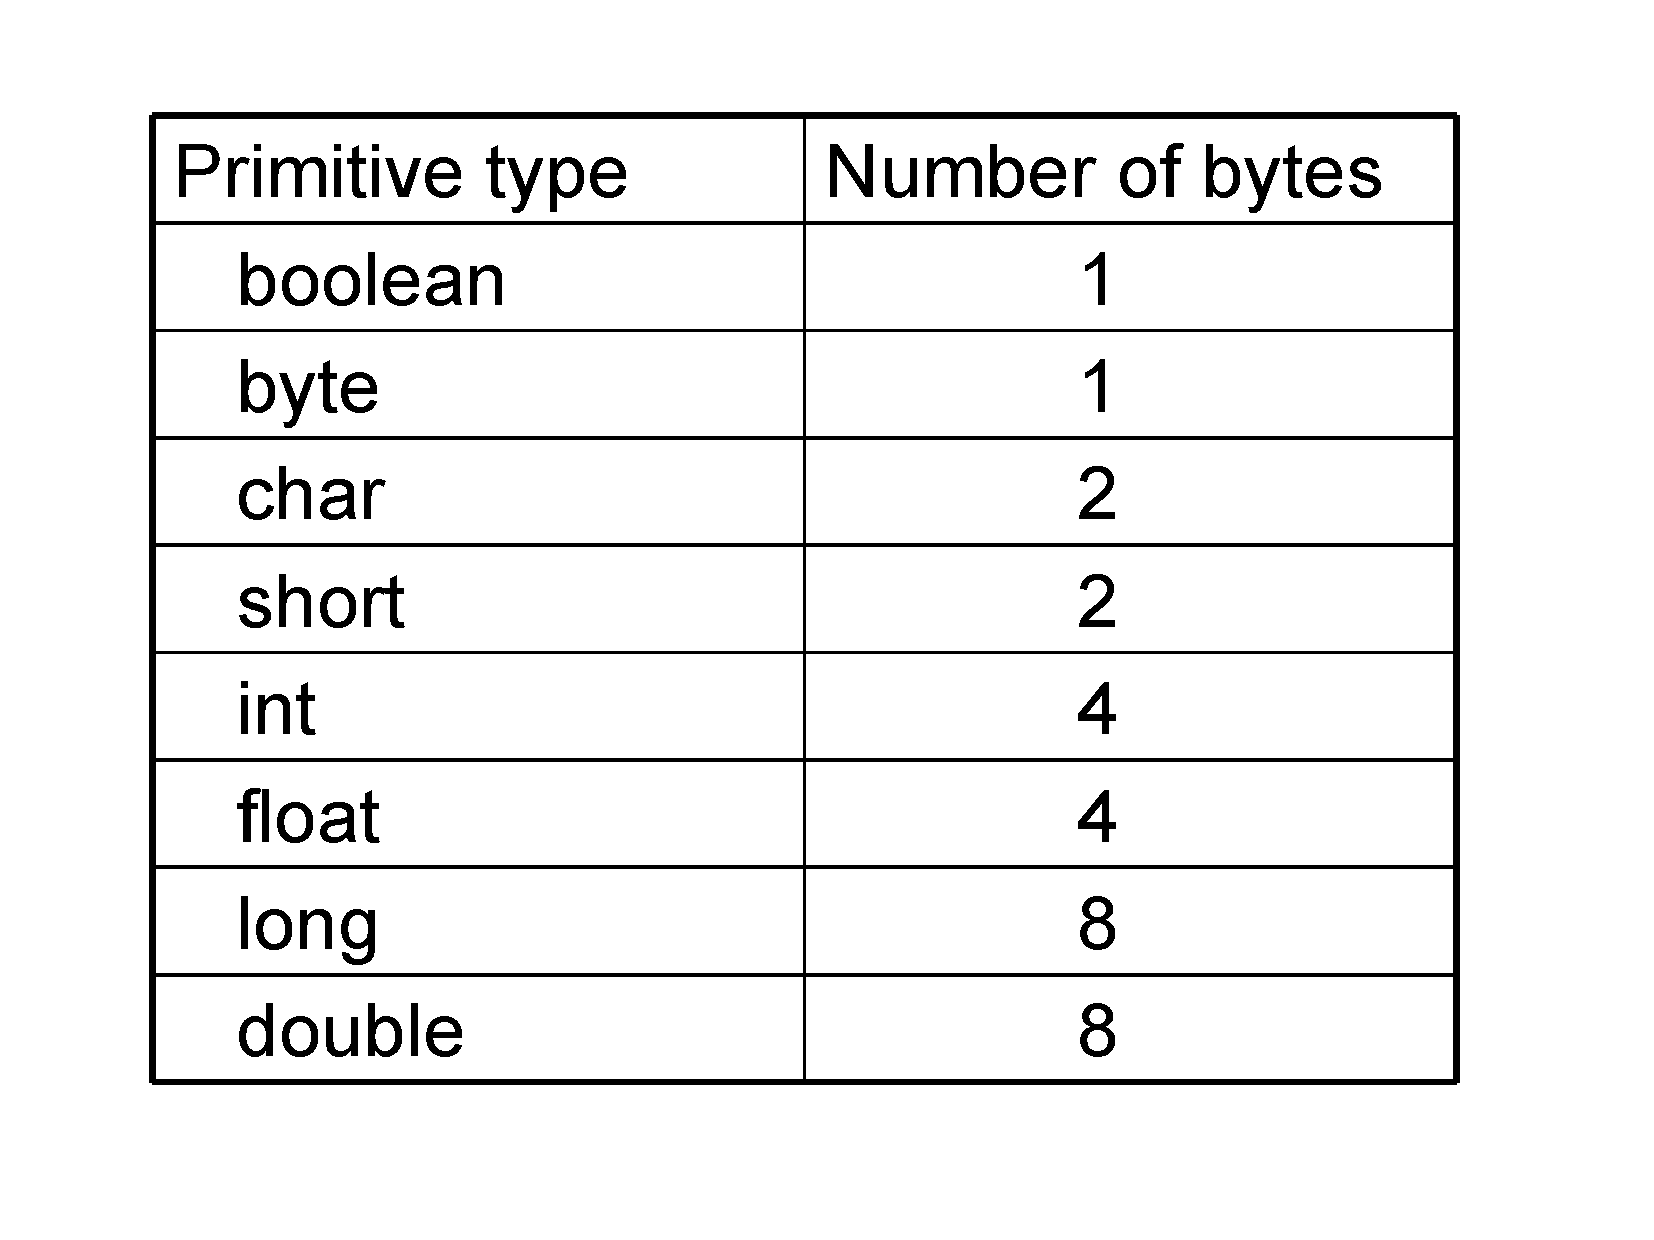
\includegraphics[width=.50\textwidth]{Figures/chapter4/primitive-byte-sizes.pdf}
\begin{tabular}{lc} \toprule
	Primitive data type & Number of bytes \\ \midrule
	boolean, byte & 1 \\
%	byte & 1 \\ \midrule
	char, short & 2 \\
	%short & 2 \\ \midrule
	int, float & 4 \\
%	float & 4 \\ \midrule
	long, double & 8 \\
%	double & 8 \\
	\bottomrule
\end{tabular}
 % 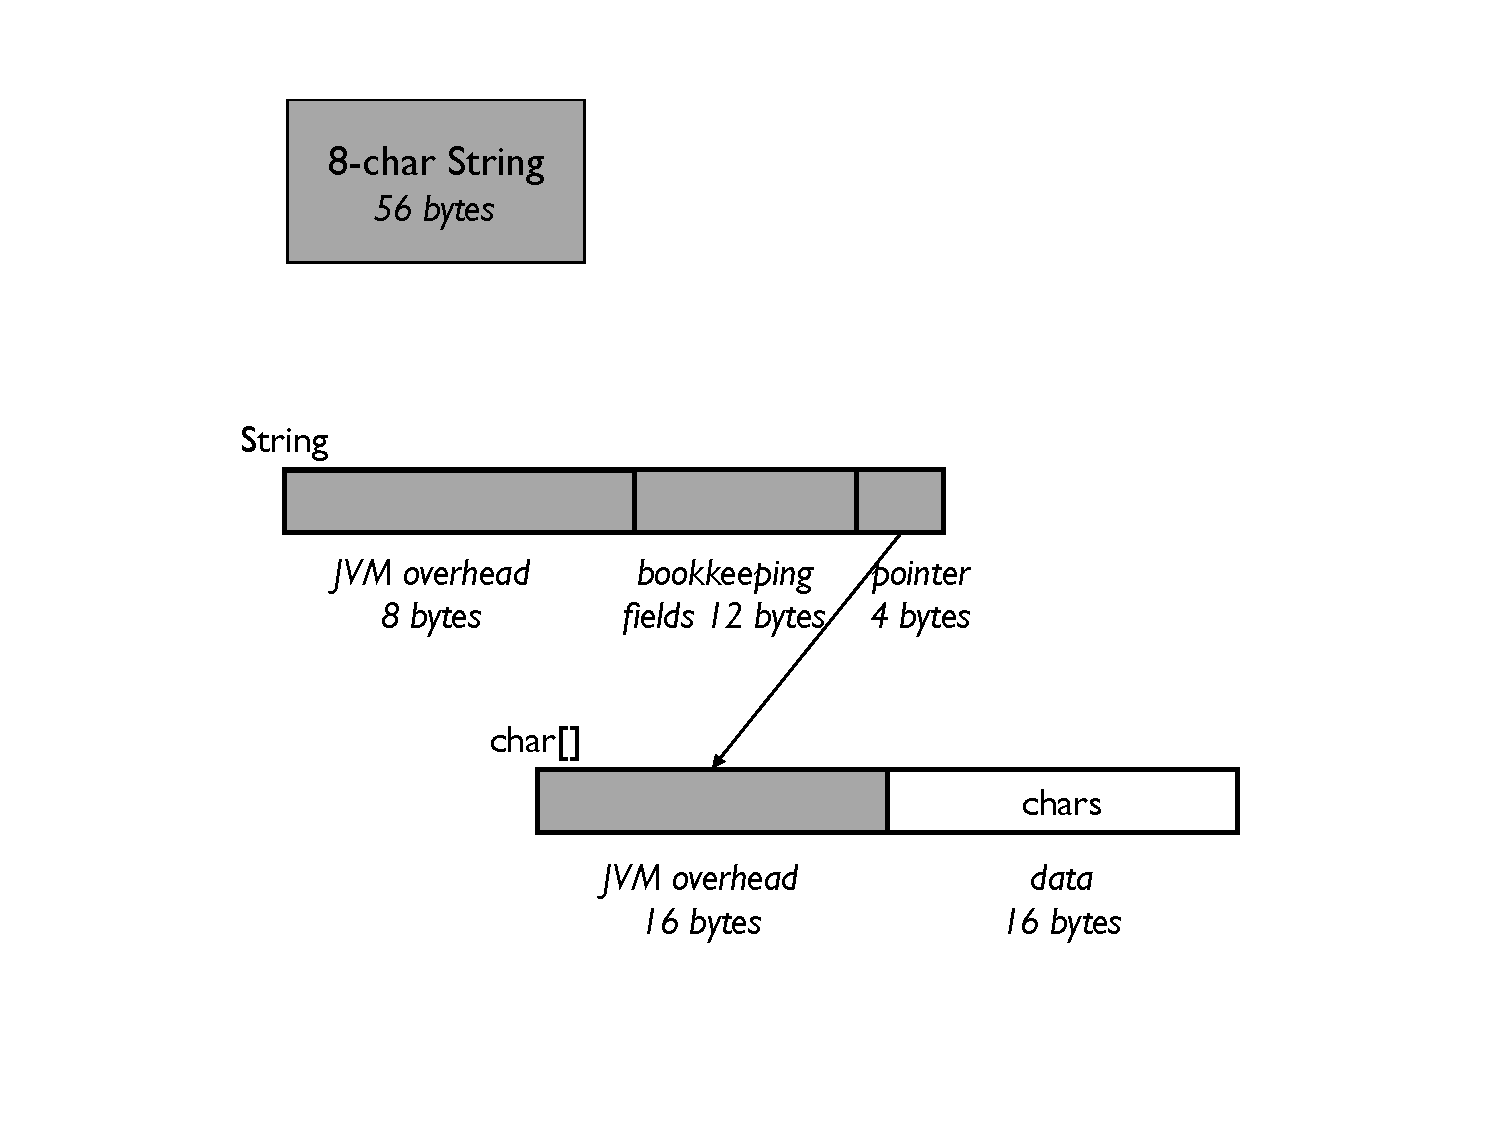
\includegraphics{eight-char-string}
  \caption{The number of bytes needed to store primitive data.}
  \label{tab:primitive-sizes}
\end{table}

Objects are bigger than the sum of their fields, and object sizes depend on the specific JRE implementation. First, the JRE allocates a header with each object that stores information such as the object's class, an identity hashcode, a monitor used for locking, and various flags. For array objects, the header has an additional integer to store the number of array elements. Secondly, JREs require objects to be aligned on address boundaries. To illustrate how implementations may differ, Table~\ref{tab:object-overhead} gives costs for two JREs, SUN Java 6 (update 14) and IBM Java 6 (J9 SR4) JRE. It is important to keep in mind that these costs are for 32-bit architectures, and JRE-specific costs are subject to change in future releases.
\begin{table}
  \centering
 %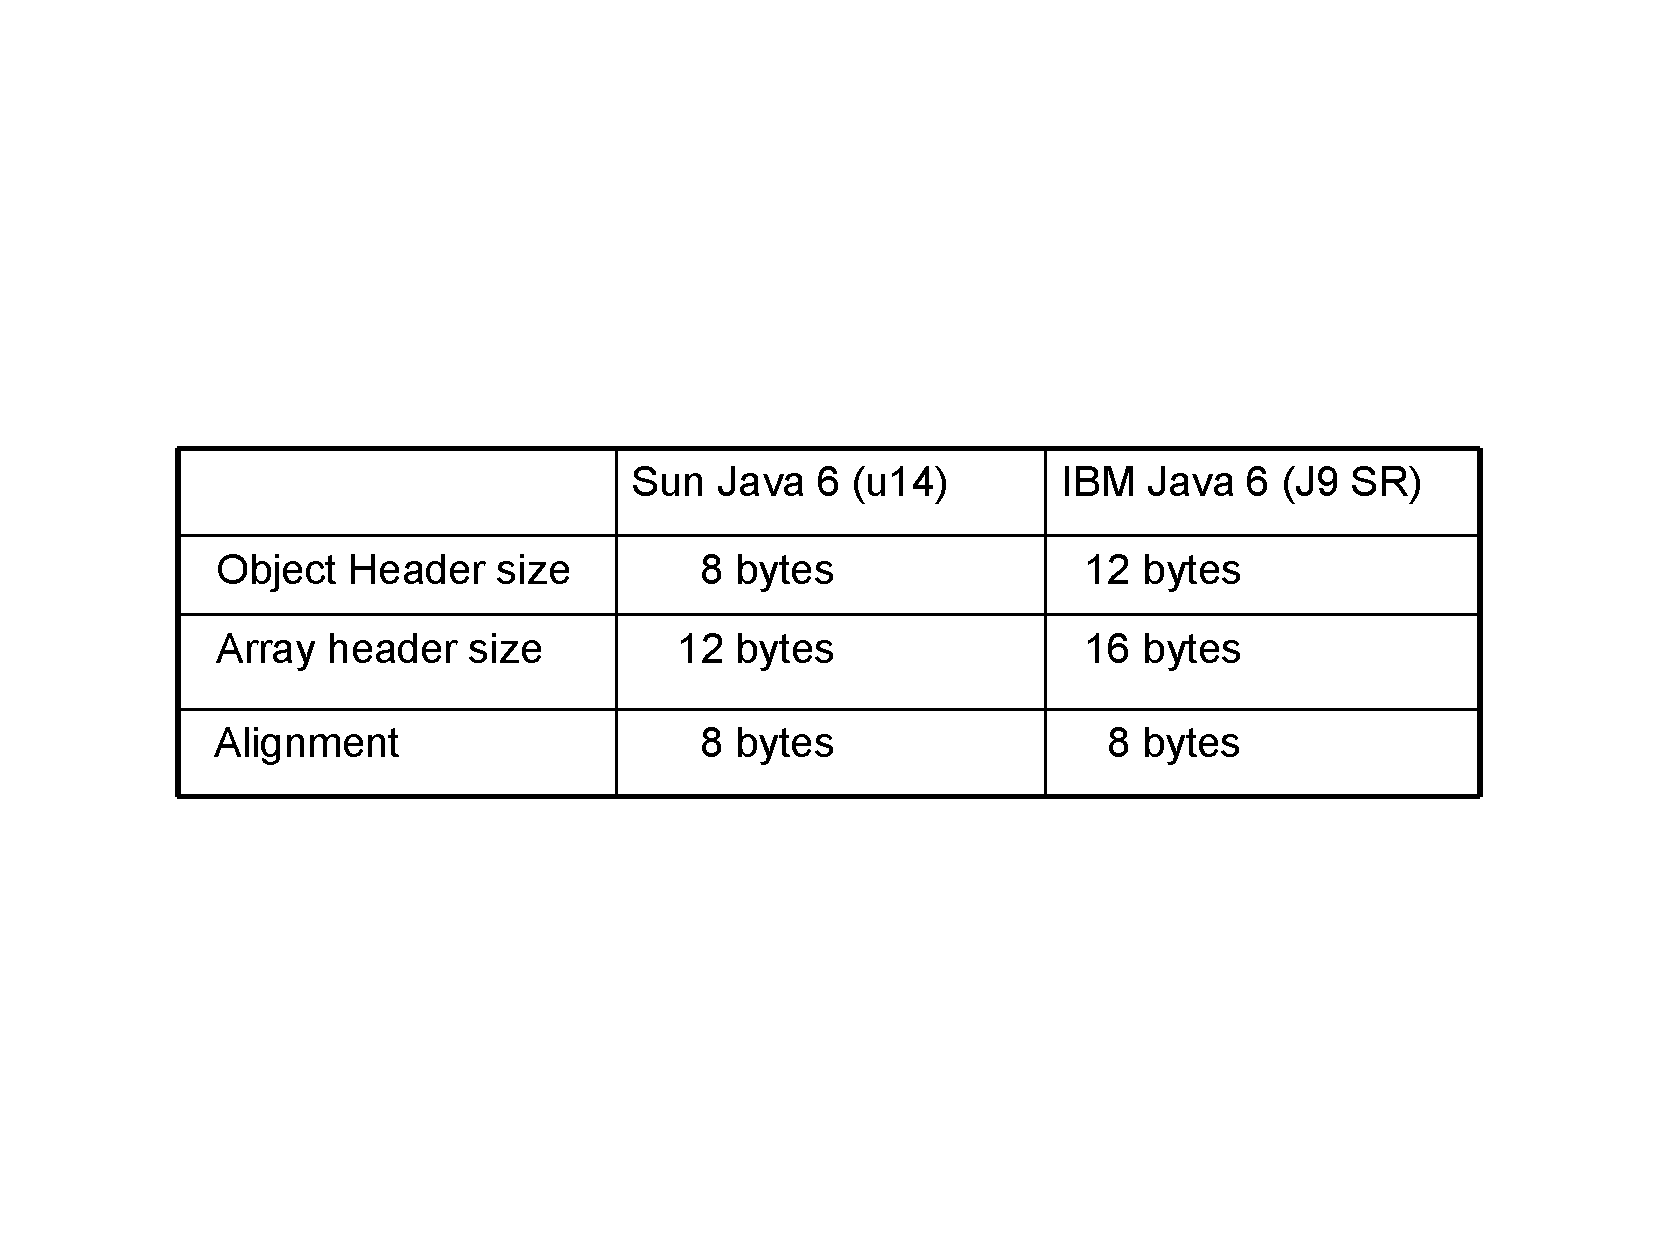
\includegraphics[width=.70\textwidth]{Figures/chapter4/object-overhead.pdf}
 % 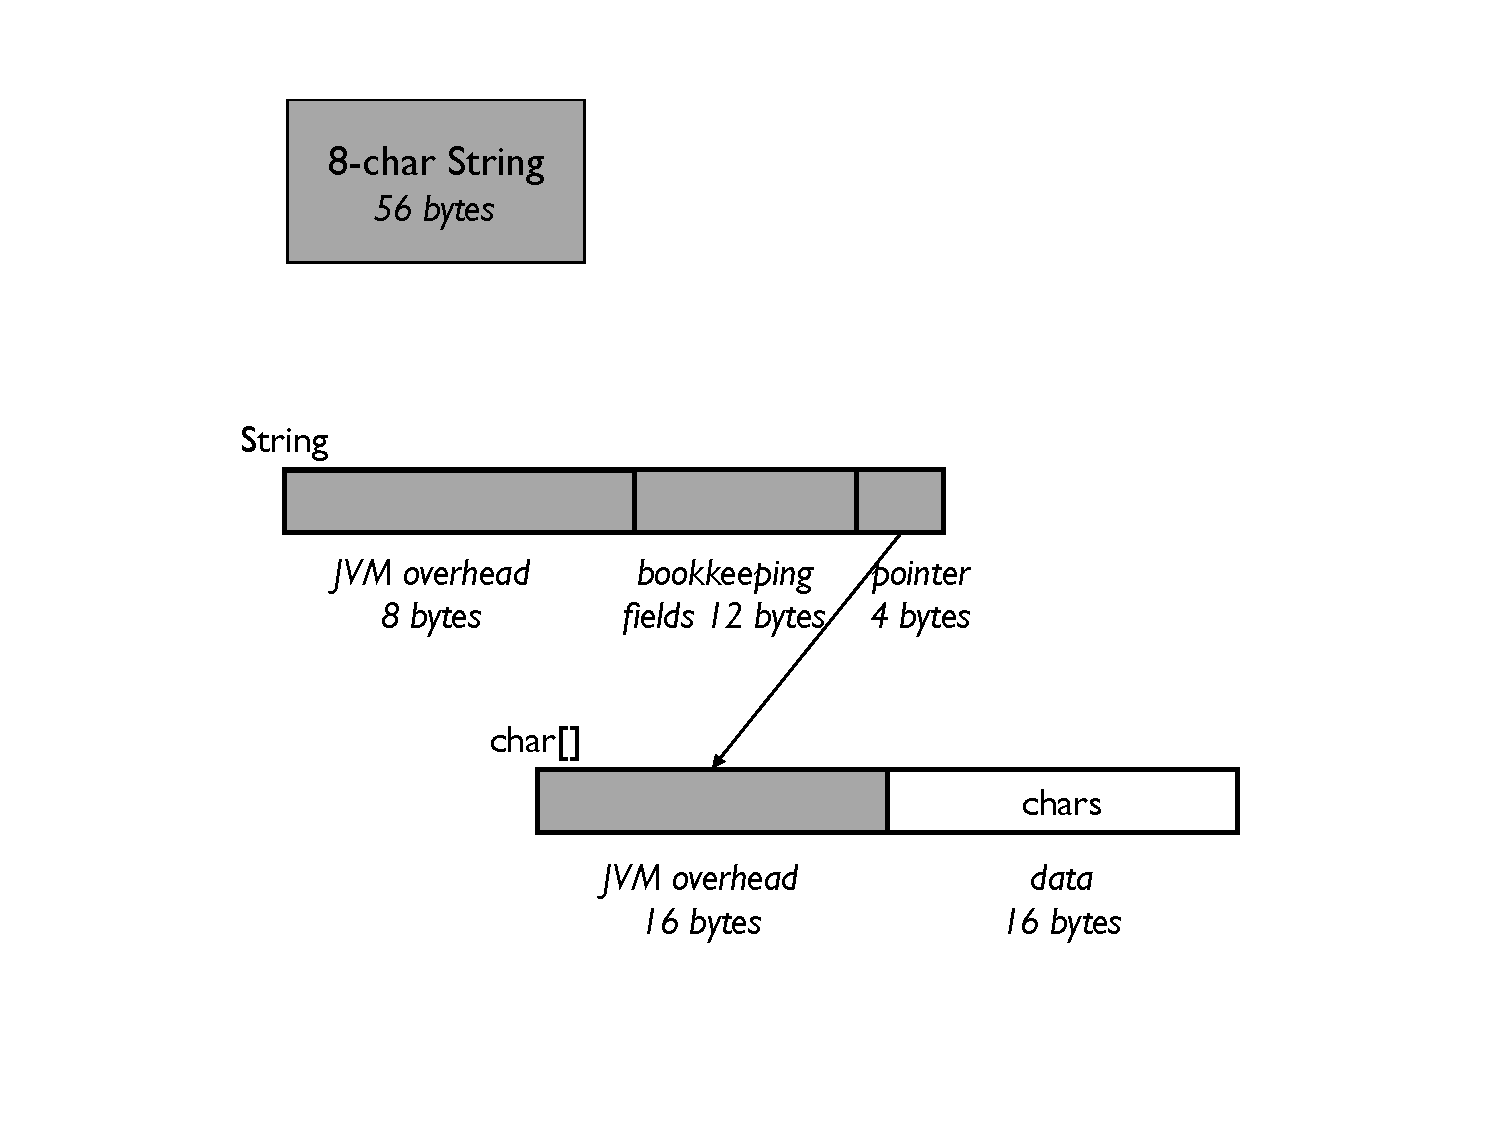
\includegraphics{eight-char-string}
 \begin{tabular}{lll} \toprule
 	& Sun Java 6 (u14) & IBM Java 6 (SR4) \\ \midrule
 	Object Header size & 8 bytes & 12 bytes \\
 	Array Header size & 12 bytes & 16 bytes \\
 	Object alignment & 8 byte boundary & 8 byte boundary \\
 	\bottomrule
 \end{tabular}
  \caption{Object overhead for both the Sun and IBM JREs.}
  \label{tab:object-overhead}
\end{table} 
   %The Sun JVM allocates 8 bytes per object header, and the IBM JVM allocates 12 bytes per header. 
   
Boxed scalars, which are objects with a single primitive data type field, are the simplest kind of  object. Since both the Sun and IBM JREs allocate objects on 8-byte boundaries, the size of an object must be a multiple of 8. For both JREs, a boxed scalar is at least 16 bytes.  Table~\ref{tab:boxed-scalar-sizes} gives the sizes of boxed scalars.

\begin{table}
  \centering
%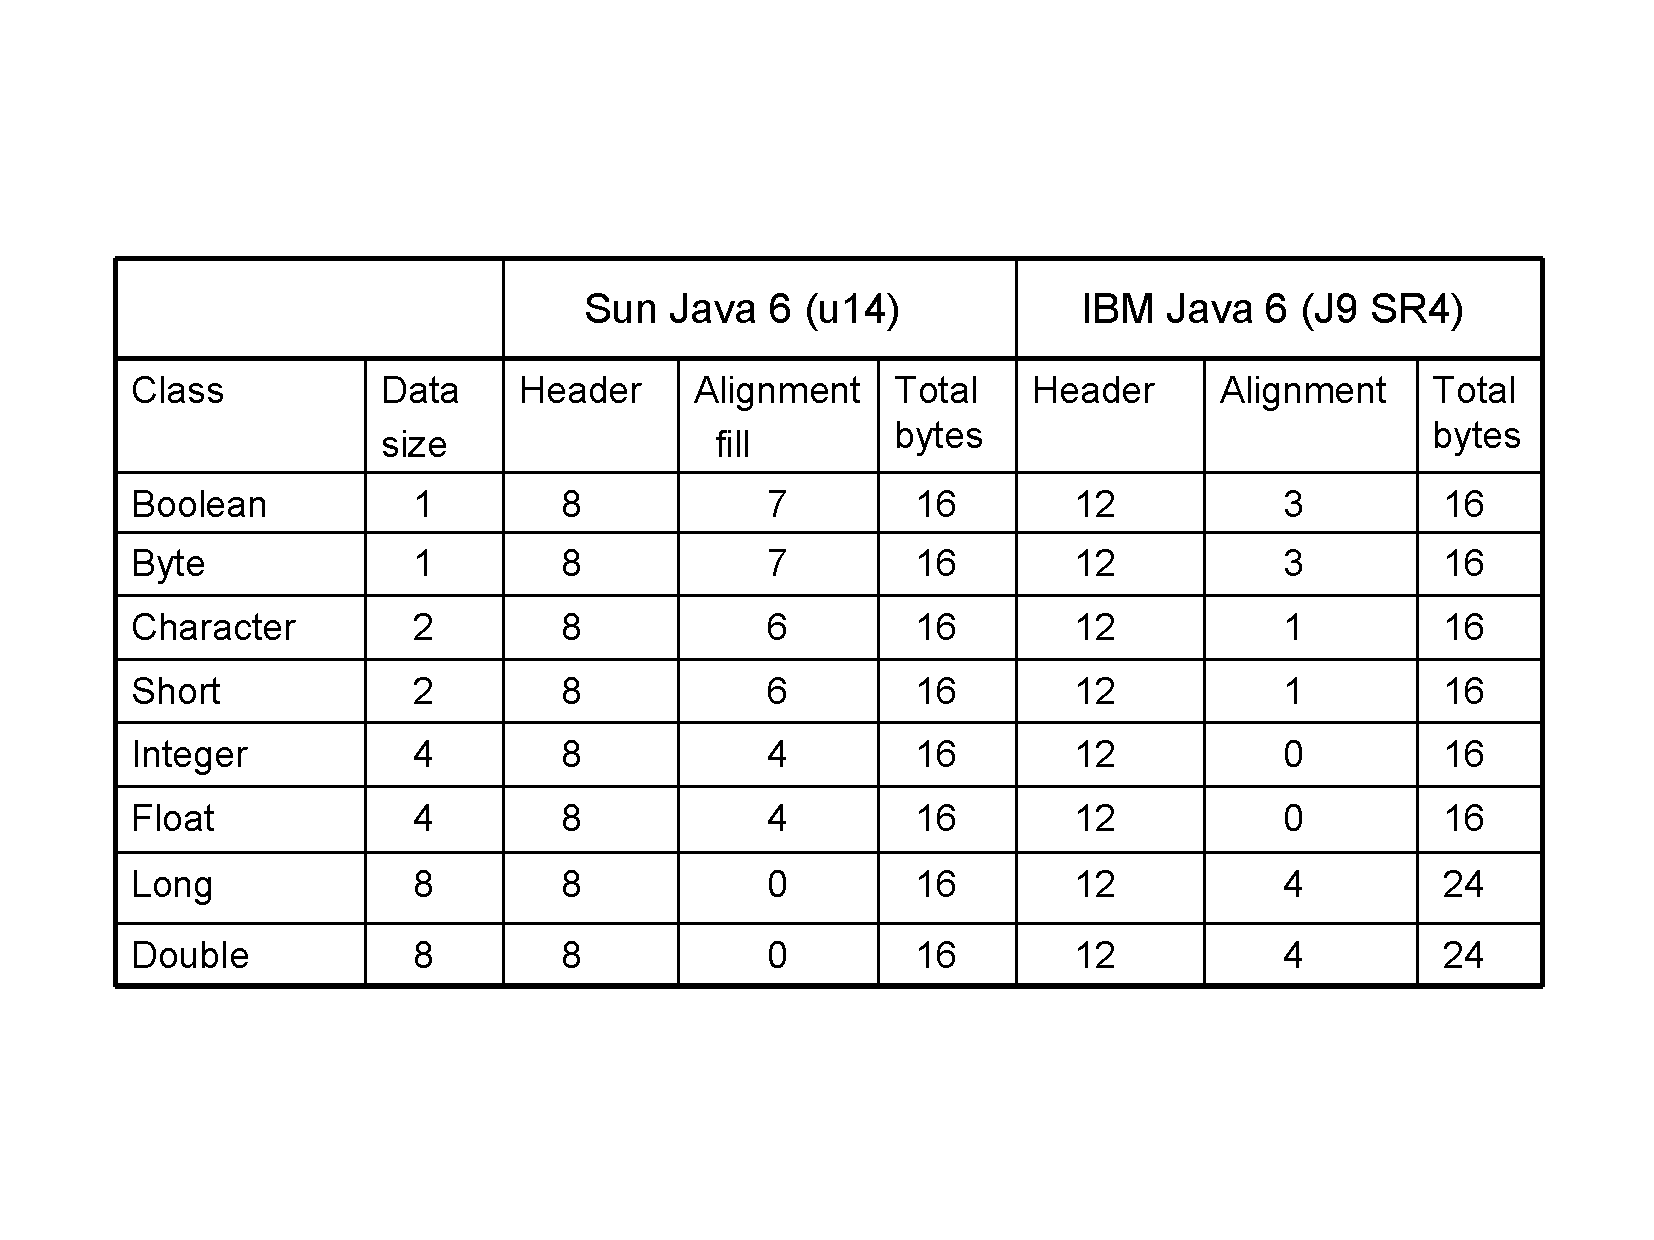
\includegraphics[width=.70\textwidth]{Figures/chapter4/boxed-scalar-sizes.pdf}
	\begin{tabular}{lccccccc} \toprule
    	& & \multicolumn{3}{c}{Sun Java 6 (u14)} & \multicolumn{3}{c}{IBM Java 6
    	(SR4)} \\ \cmidrule(r){3-5} \cmidrule(l){6-8}
    	%
    	Class & \shortstack[c]{Data\\Size} & Header & \shortstack{Align-\\ment
    	fill} & \shortstack[c]{Total\\bytes} & Header & \shortstack{Align-\\ment
    	fill} & \shortstack[c]{Total\\bytes} \\ \midrule {\small Boolean, Byte} &
    	1 & 8 & 7 & 16 & 12 & 3 & 16 \\ {\small Character, Short} & 2 & 8 & 6 & 16 & 12 & 1 & 16 \\
    	{\small Integer, Float} & 4 & 8 & 4 & 16 & 12 & 0 & 16 \\
    	{\small Long, Double} & 8 & 8 & 0 & 16 & 12 & 4& 24 \\
		\bottomrule
	\end{tabular}
  \caption{The sizes of boxed scalar objects.}
  \label{tab:boxed-scalar-sizes}
\end{table}
 
For objects with more than one primitive data field, computing object sizes is a bit more complicated. The hardware often imposes alignment restrictions on specific data types, for example, requiring integer fields to be aligned on 4 byte boundaries. Field alignment can introduce more padding.
 
\begin{example}[Simple employee class.]
Consider a \texttt{SimpleEmployee} class with all primitive fields. The comments show the primitive data size of each field:
\begin{verbatim}
      class SimpleEmployee {
        int hoursPerWeek;        // 4 bytes 
        boolean exempt;          // 1 bytes
        double salary;           // 8 bytes
        char jobCode;            // 2 bytes
        int yearsOfService;      // 4 bytes	
}
\end{verbatim}
If the fields are laid out one after the other the \texttt{double} field \texttt{salary} would begin on a 5-byte boundary, which is not allowed. Either the \texttt{exempt} field must be padded, or the fields must be rearranged to fill in the empty spaces. The specific JRE implementation may differ.
\end{example}
The Sun JRE does a good job rearranging and packing fields, so that you can assume each field is the size needed to store its primitive data type. With the Sun JRE, the size of a \texttt{SimpleEmployee} object is 32 bytes:
\begin{verbatim}
                      fields   + header          round up    
                   (4+1+8+2+4) +   8     =  27      32
\end{verbatim} 

In contrast, the IBM JRE makes all fields in non-array objects either 4 or 8 bytes.  Here is the \texttt{SimpleEmployee} class with field sizes adjusted for the IBM JRE. 
\ttfamily
\begin{verbatim} 
			class SimpleEmployee {
        int hoursPerWeek;        // 4 bytes
        boolean exempt;          // 4 byte
        double salary;           // 8 bytes
        char jobCode;            // 4 bytes
        int yearsOfService;      // 4 bytes
			}
\end{verbatim}
\normalfont
The size of a \texttt{SimpleEmployee} object with the IBM JRE is 40 bytes:
\begin{verbatim}
               fields   +  header          round up
            (4+4+8+4+4) +   12   = 36,       40
\end{verbatim}
For arrays, both the Sun and IBM JRE pack the data fields on byte boundaries.
\callout{callout:minimum-size-estimation-rule}{Estimating Object Sizes}{
The size of an object can be estimated as follows:
\begin{enumerate}
\item Add up the sizes of all of the fields in the object's class and all of its superclasses.
\item Add the size of the object header to the result.
\item Round up the result to the next multiple of the object alignment.
\end{enumerate}
The object header size, the object alignment, and the sizes of the fields depend on the JRE. For example, the JRE may pack fields to obtain the minimum possible size (e.g. Sun), or align fields on word boundaries (e.g. IBM). Array fields are always packed.
}

When objects are small, For objects with primitive data only, the bloat factor decreases as the object size increases. The overhead cost consists of a fixed object header cost and a bounded alignment cost, which are amortized when the object is big.  For example, for the Sun JRE, the bloat factors for the boxed scalars with one field range from 94\% for a \texttt{Boolean} down to 50\% for a \texttt{Double}.  The bloat factor for a \texttt{SimpleEmployee} is 46\%.  The bloat factor for an array of 100 \texttt{int}s is insignificant. This is not the case for objects with other kinds of overhead, like pointers.

\section{The Cost of Delegation}

The \texttt{Employee} class is not a very realistic example, since it has only primitive fields. Usually, a class has some fields that are objects.  In Java, a field of type \texttt{ObjectType} is implemented using \textit{delegation}, that is, the field stores a reference to another object of type \texttt{ObjectType}. On 32-bit architectures, a pointer is 4 bytes. You can calculate the size of any object as described in in Section~\ref{sec:CostOfObjects}, plugging in 4 bytes for each reference field. Unless otherwise stated, the following examples assume the Sun JRE. 
\begin{example}[Employee class with delegation]
Here is a more realistic employee class with several reference fields. An employee now has a name, which is a \texttt{String}, and a start date, which is a \texttt{Date}. The type of \texttt{salary} has been changed from \texttt{double} to \texttt{BigDecimal}. \texttt{BigDecimal} avoids potential roundoff errors.
\ttfamily
\begin{verbatim} 
			class EmployeeWithDelegation {
        int hoursPerWeek;           // 4 bytes
        String name;                // 4 bytes
        BigDecimal salary;          // 4 bytes
        Date startDate;             // 4 bytes
        boolean exempt;             // 1 byte
        char jobCode;               // 2 bytes
        int yearsOfService;         // 4 bytes
			}
\end{verbatim}
\normalfont
The minimum size of an \texttt{EmployeeWithDelegation} object is 32 bytes:
\begin{verbatim}
                (4+4+4+4+1+2+4) + 8 = 31, rounds up to 32 bytes
\end{verbatim} 
\end{example}

While an instance of the \texttt{EmployeeWithDelegation} class is a single 32 byte object, an entire employee, including name, salary, and start date consists of five objects. Two of these objects are used to store the name. (Recall from Section~\ref{sec:bloat-def} that a string is represented by a wrapper \texttt{String} object and a \texttt{char} array.) The memory layout for a specific employee ``John Doe" is shown in Figure~\ref{fig:employee-status}. 
 \begin{figure}
  \centering
 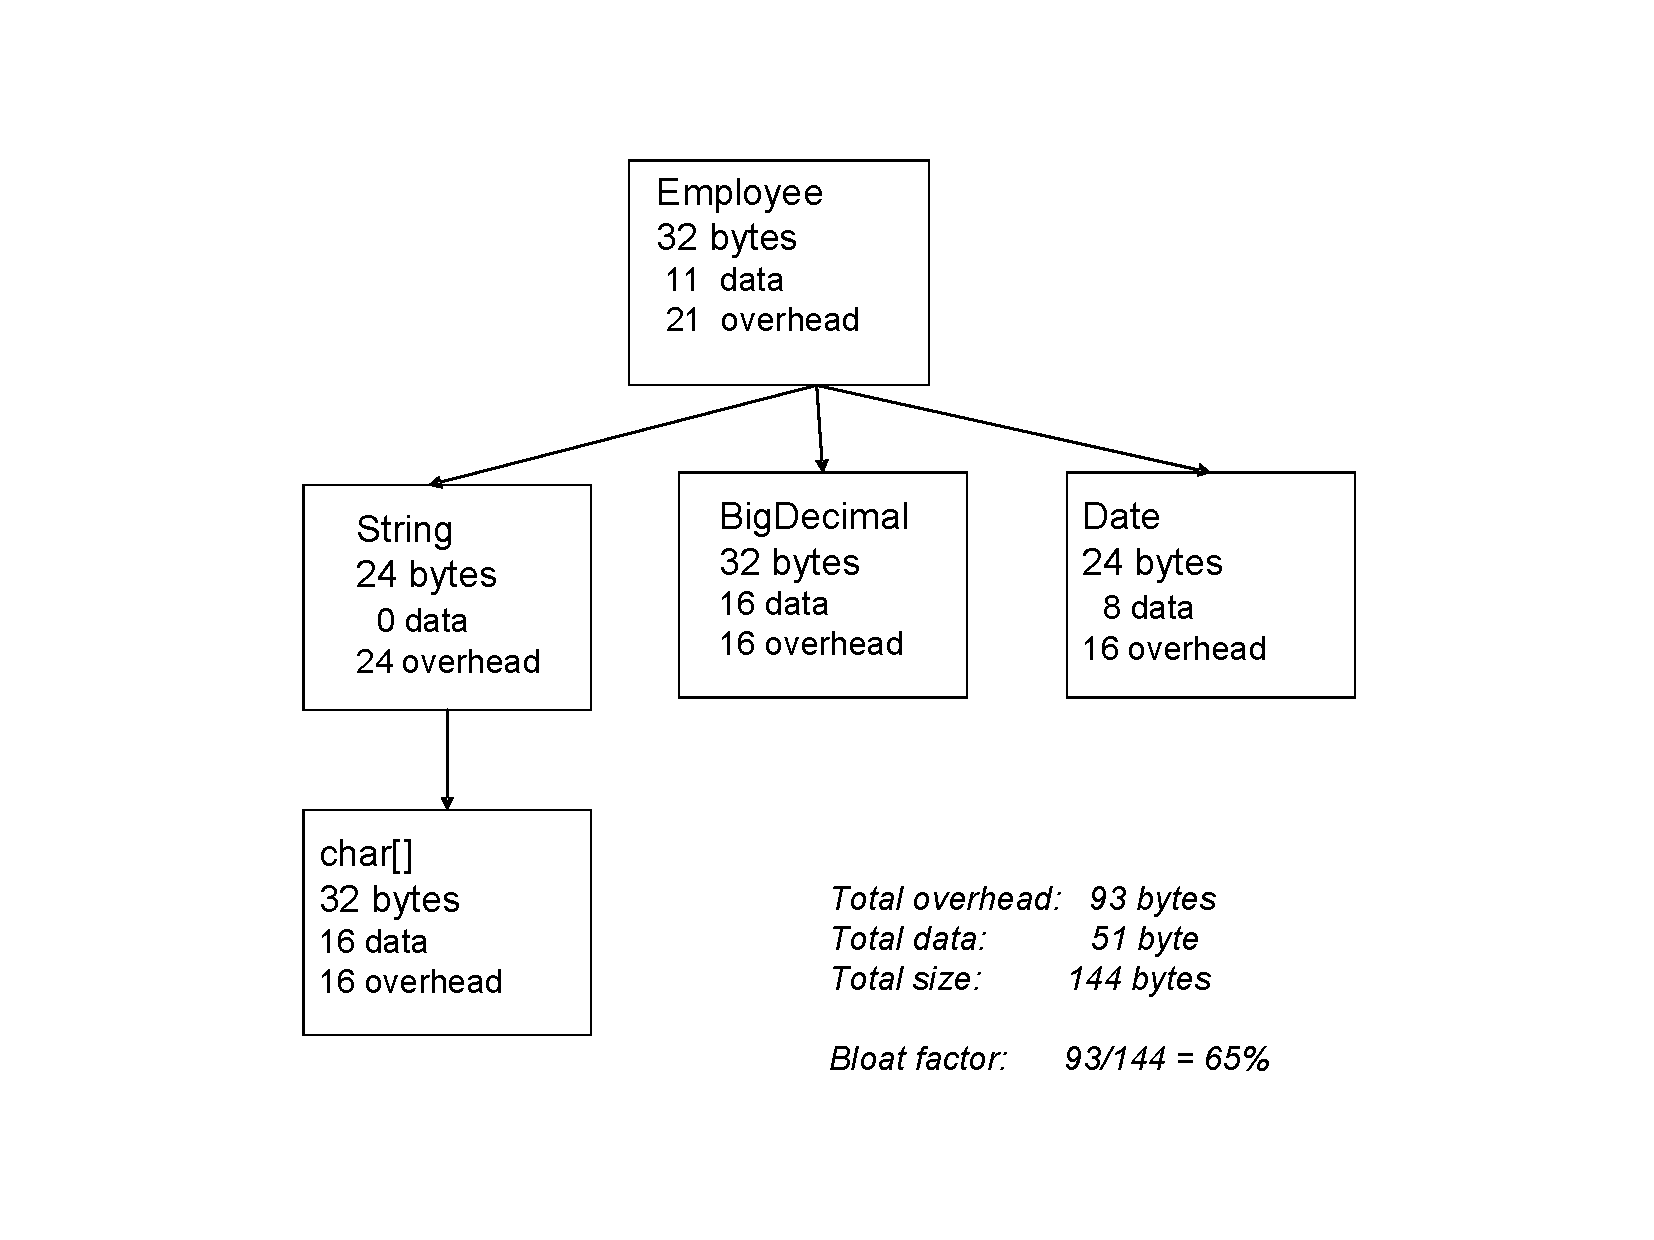
\includegraphics[width=.60\textwidth]{Figures/chapter4/employee-status.pdf}
 % 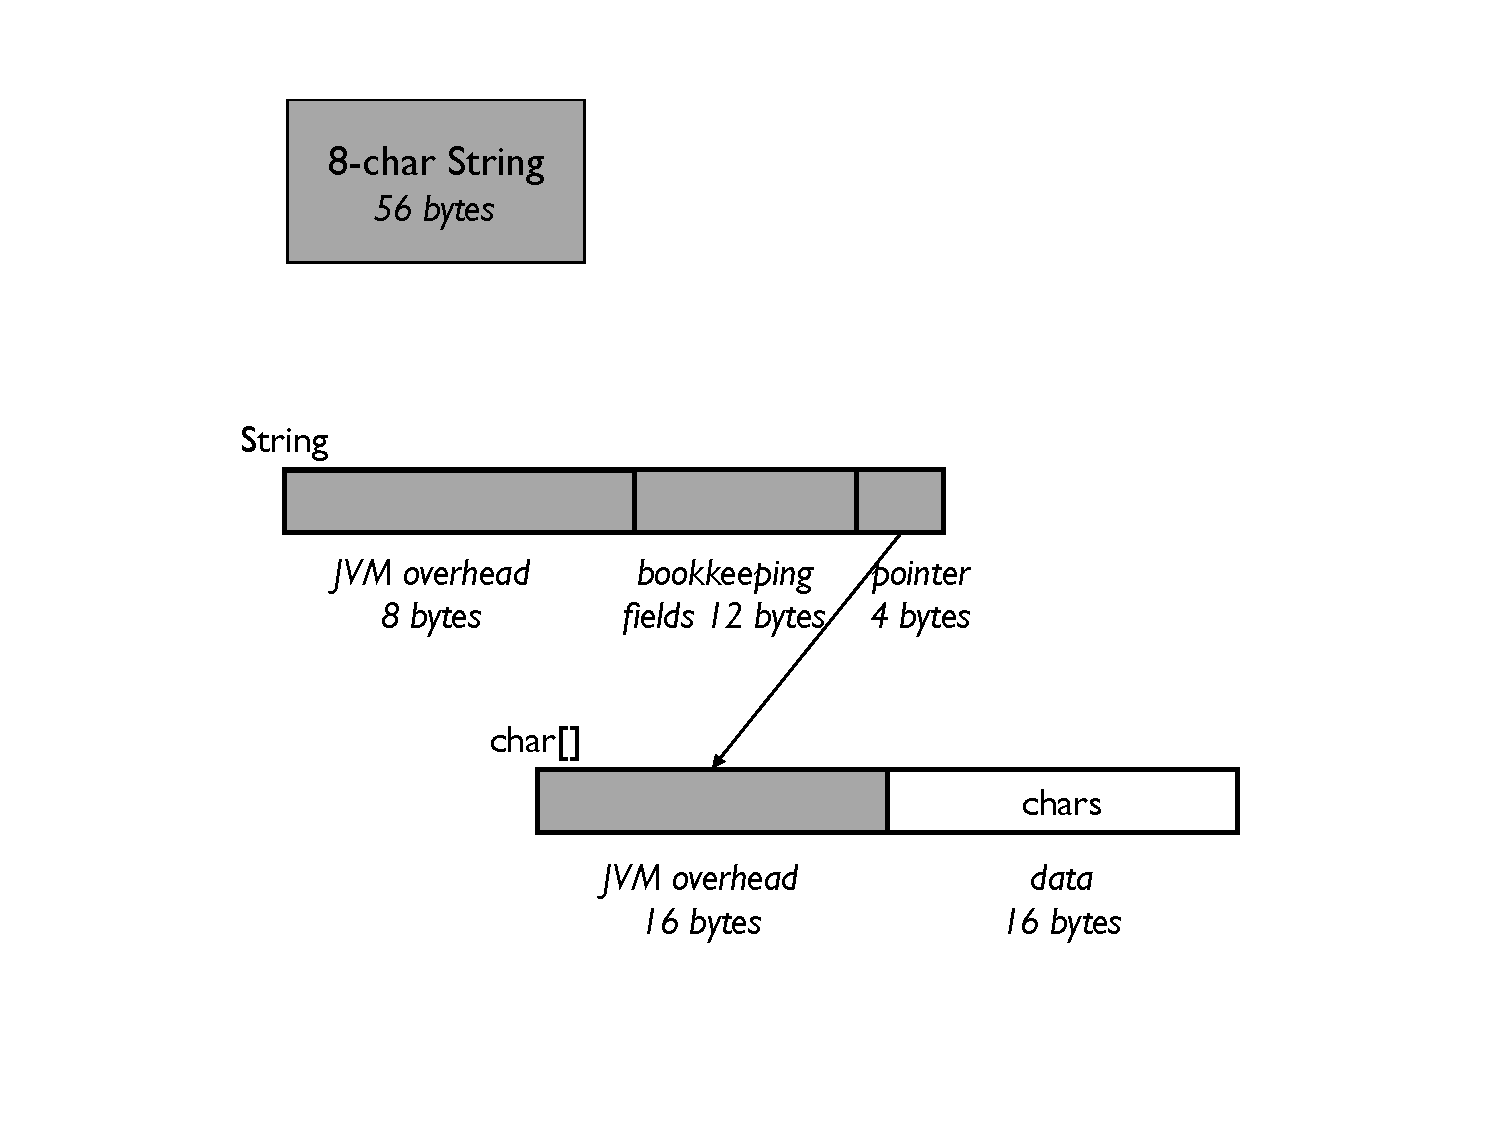
\includegraphics{eight-char-string}
  \caption{The memory layout for an employee ``John Doe"}
  \label{fig:employee-status}
\end{figure}

A comparion of a \texttt{EmployeeWithDelegation} object with a \texttt{SimpleEmployee} object from Section~\ref{sec:CostOfObjects} shows that the size has increased from 32 to 144 bytes, and the bloat factor has increased from 46\% to 65\%. There is more information stored in the new version, so it is no surprise that it is bigger. The increase in the bloat factor is more significant. Delegation increases memory bloat. Delegation introduces additional object headers, a pointer for each delegated object, and empty pointer slots for uninitialized object fields. Delegation may also force additional alignment costs, since each new delegated object has to be aligned to an 8-byte boundary. 

In the spirit of keeping things simple, Java does not allow you to nest objects inside other objects, to build a single object out of other objects. You cannot nest an array inside an object, and you cannot store objects directly in an array.  You can only point to other objects. Even the basic data type \texttt{String} consists of two objects. This means that delegation is pervasive in Java programs, and it is difficult to avoid a high level of delegation overhead. Single inheritance is the only language feature that can be used instead of delegation to compose two object, but single inheritance has limited flexibility.  In contrast, C++ has many different ways to compose objects. C++ has single and multiple inheritance, union types, and variation. C++ allows you to have \texttt{struct} fields, you can put arrays inside of structs, and you can also have an array of structs.  

Because of the design of Java, there is a basic delegation cost that is hard to eliminate it. This is the cost of object-oriented programming in Java. While it is hard to avoid this basic delegation cost, it is important not to make things a lot worse, as discussed in the next section. 

\section{Fine-Grained Data Models}
\label{fine-grained-data-models}

The Java language makes it hard to avoid delegation. Programmer choices also impact delegation costs.  The current software engineering culture tends to promote delegation, and for good reasons. Delegation provides a loose coupling of objects, making refactoring and reuse easier. Replacing inheritance by delegation is often recommended, especially if the base class has extra fields and methods that the subclass does not need. In languages with single inheritance, once you have used up your inheritance slot, it becomes hard to refactor your code. Therefore, delegation can be more flexible than inheritance for implementing polymorphism. However, overly fine-grained data models can be expensive both in execution time and memory space. 

There is no simple rule that can always be applied to decide when to use delegation. Each situation has to be evaluated in context, and there may be tradeoffs among different goals. To make an informed decision, it is important to know what the costs are.

\begin{example}[Employee emergency contact] 
Suppose an emergency contact is needed for each employee. An emergency contact is a person along with a preferred method to reach her.  The preferred method can be email, cell phone, work phone, or home phone. All contact information for the emergency contact person must be stored, just in case the preferred method does not work in an actual emergency. 
\end{example}
Here are class definitions for an emergency contact, written in a highly delegated style that is not uncommon in real applications. 

\ttfamily
\begin{verbatim} 
			class EmployeeWithEmergencyContact {
        ...
        EmergencyContact contact;
			}
			
			class EmergencyContact {
        ContactPerson contact;
        ContactMethod preferredContact;
			}
			
			class ContactPerson {
        String name;
        String relation;
        EmailAddress email;
        PhoneNumber phone;
        PhoneNumber cell;
        PhoneNumber work;
			}
			
			class ContactMethod {
        ContactPerson owner;
			}
			
			class PhoneNumber extends ContactMethod {
			  byte[] phone;
			}
			
			class EmailAddress extends ContactMethod {
        String address;
			}
			
			
\end{verbatim}
\normalfont
 \begin{figure}
  \centering
 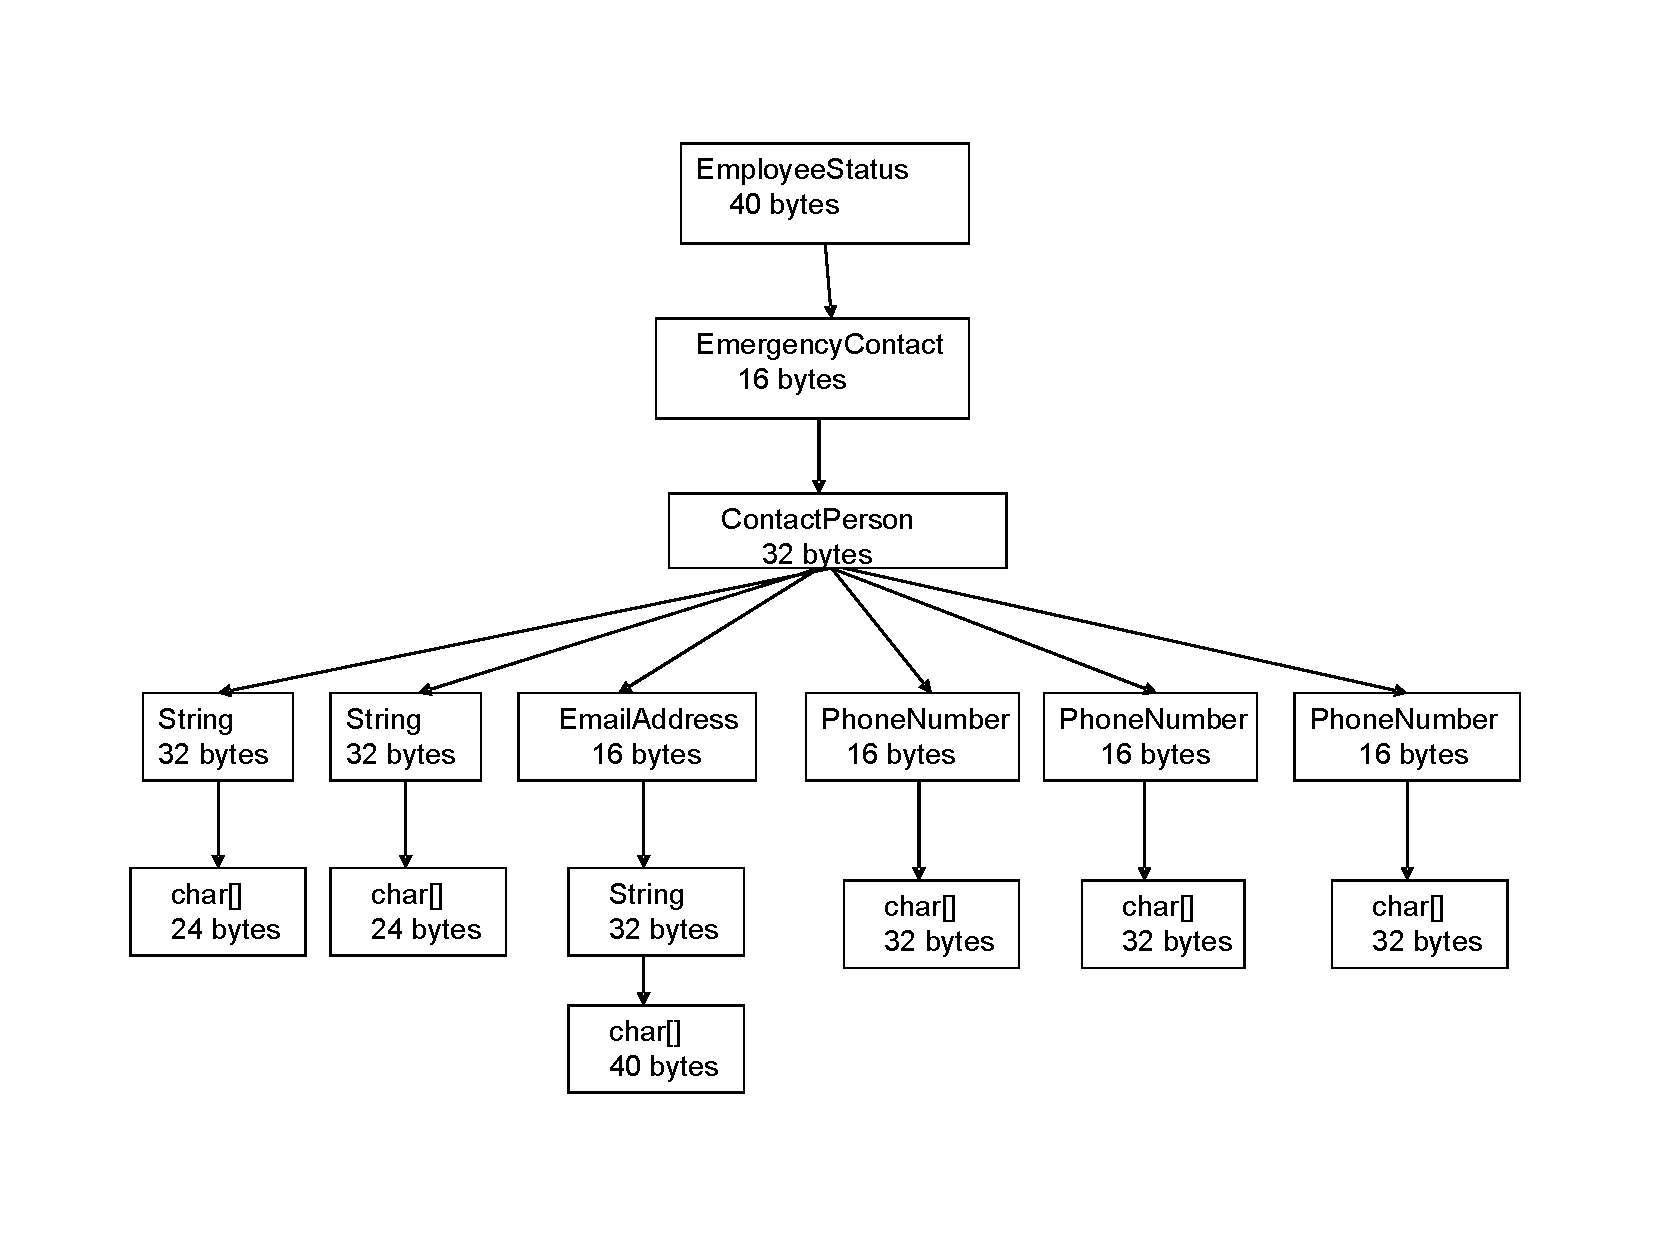
\includegraphics[width=.70\textwidth]{Figures/chapter4/employee-status-fine-grained.pdf}
 % 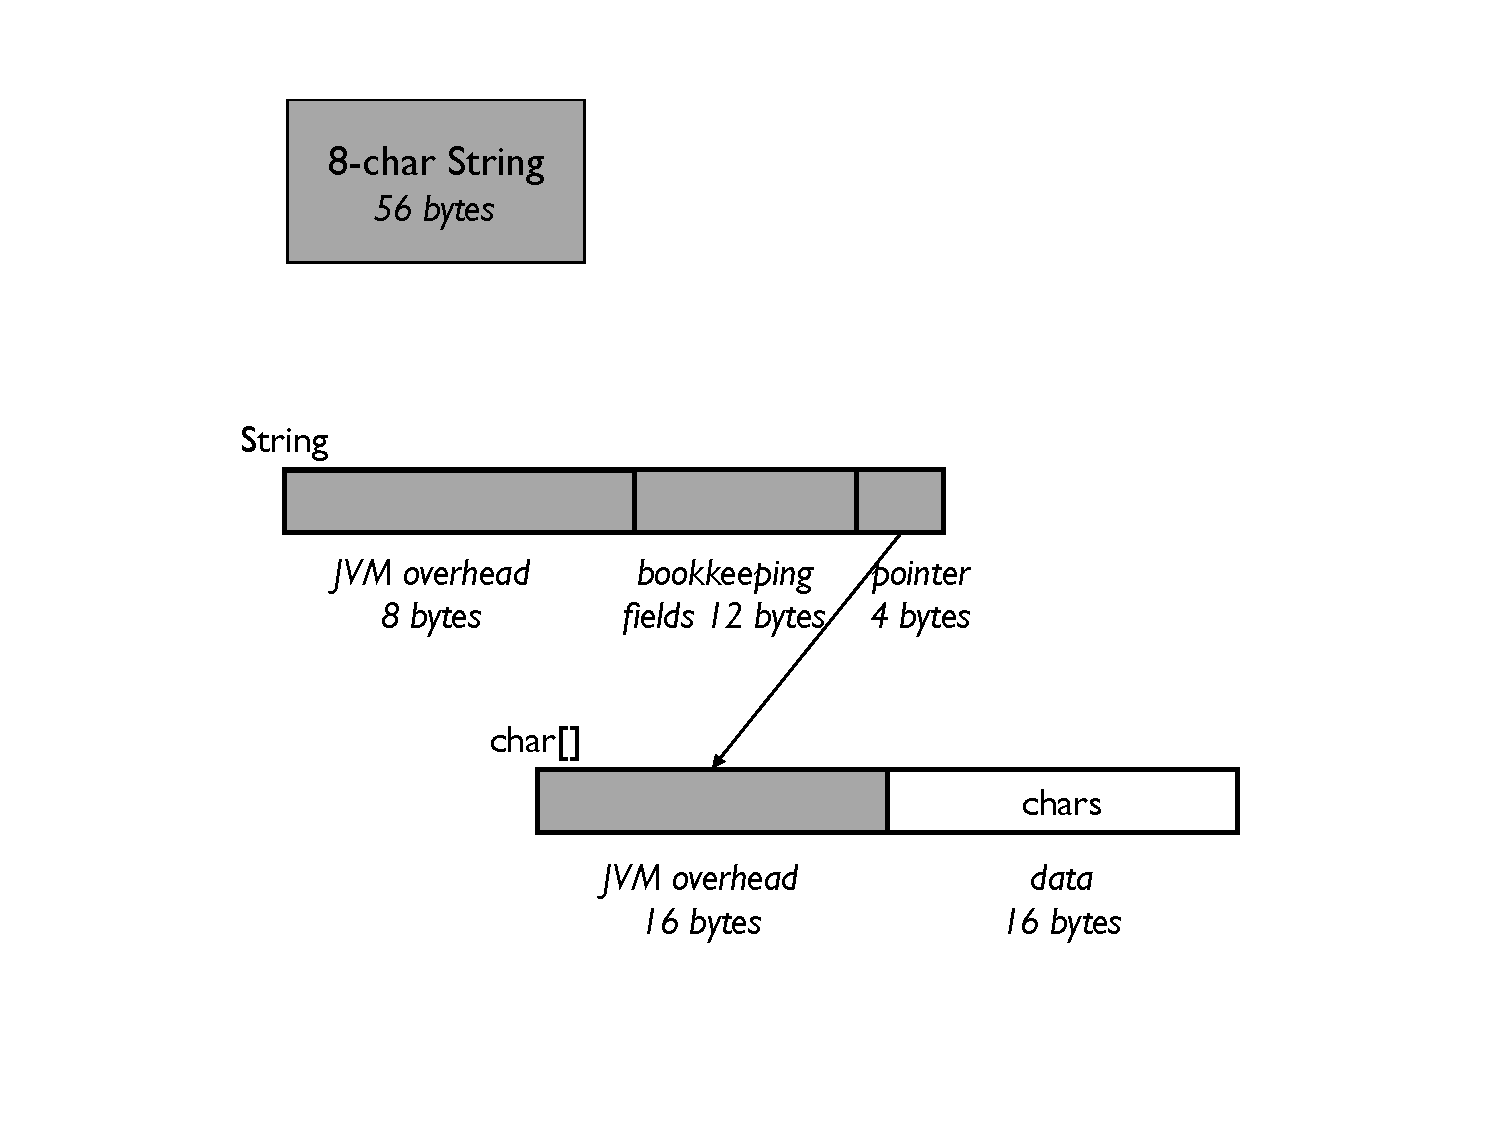
\includegraphics{eight-char-string}
  \caption{The memory layout for an employee with an emergency contact.}
  \label{fig:employee-status-fine-grained}
\end{figure}
The memory layout for a sample employee is shown in Figure~\ref{fig:employee-status-fine-grained}. There are 15 objects used to store emergency contact information, with a bloat factor of 77\%, which seems excessive. The objects are all small, containing only one or two meaningful fields, which is a symptom of an overly fine grained data model. Also, all of the data is at the bottom of object chains, 4 to 5 objects long. Refactoring can flatten this structure somewhat, undoing a few of the delegation.

One object that looks superfluous is \texttt{EmergencyContact}, which encapsulates the contact person and the preferred contact method.  
Reversing this delegation involves inlining the fields of the \texttt{EmergencyContact} class into other classes, and eliminating the \texttt{EmergencyContact} class. Here are the refactored classes:
\ttfamily
\begin{verbatim}
	class EmployeeWithEmergencyContact {
        ...
        ContactPerson contact;
			}
			
			class ContactPerson {
        String name;
        String relation;
        EmailAddress email;
        PhoneNumber phone;
        PhoneNumber cell;
        PhoneNumber work;
        ContactMethod preferredContact;
			}
\end{verbatim}
\normalfont
This change eliminates an object from Figure~\ref{fig:employee-status-fine-grained}, but it only recovers 8 bytes, since a 16 byte object is removed and \texttt{ContactPerson} is 8 bytes bigger. You can save considerably more space by inlining the four \texttt{ContactMethod} classes into the \texttt{ContactPerson} class, which removes 64 bytes of overhead. In a system with many instances of employees stored in memory, this reduction is significant. In order to make this change, the preferred contact method must be encoded somehow in \texttt{ContactPerson}.  A simple way to achieve this is to use an enumeration type field, which has the same size as a reference field, to discriminate among the different contact methods:
\ttfamily
\begin{verbatim} 
      enum PreferredContactMethod {
         EMAIL, HOME_PHONE, CELL_PHONE, WORK_PHONE;
      }
      
      class ContactPerson {
        PreferredContactMethod preferred;
        String name;
        String relation;
        String email;
        byte[] cellPhone;
        byte[] homePhone;
        byte[] workPhone;
      }		
\end{verbatim}
\normalfont
Figure~\ref{fig:refactored-fine-grain} shows the memory layout after these changes. Both the size and the bloat factor have been reduced.
 \begin{figure}
  \centering
 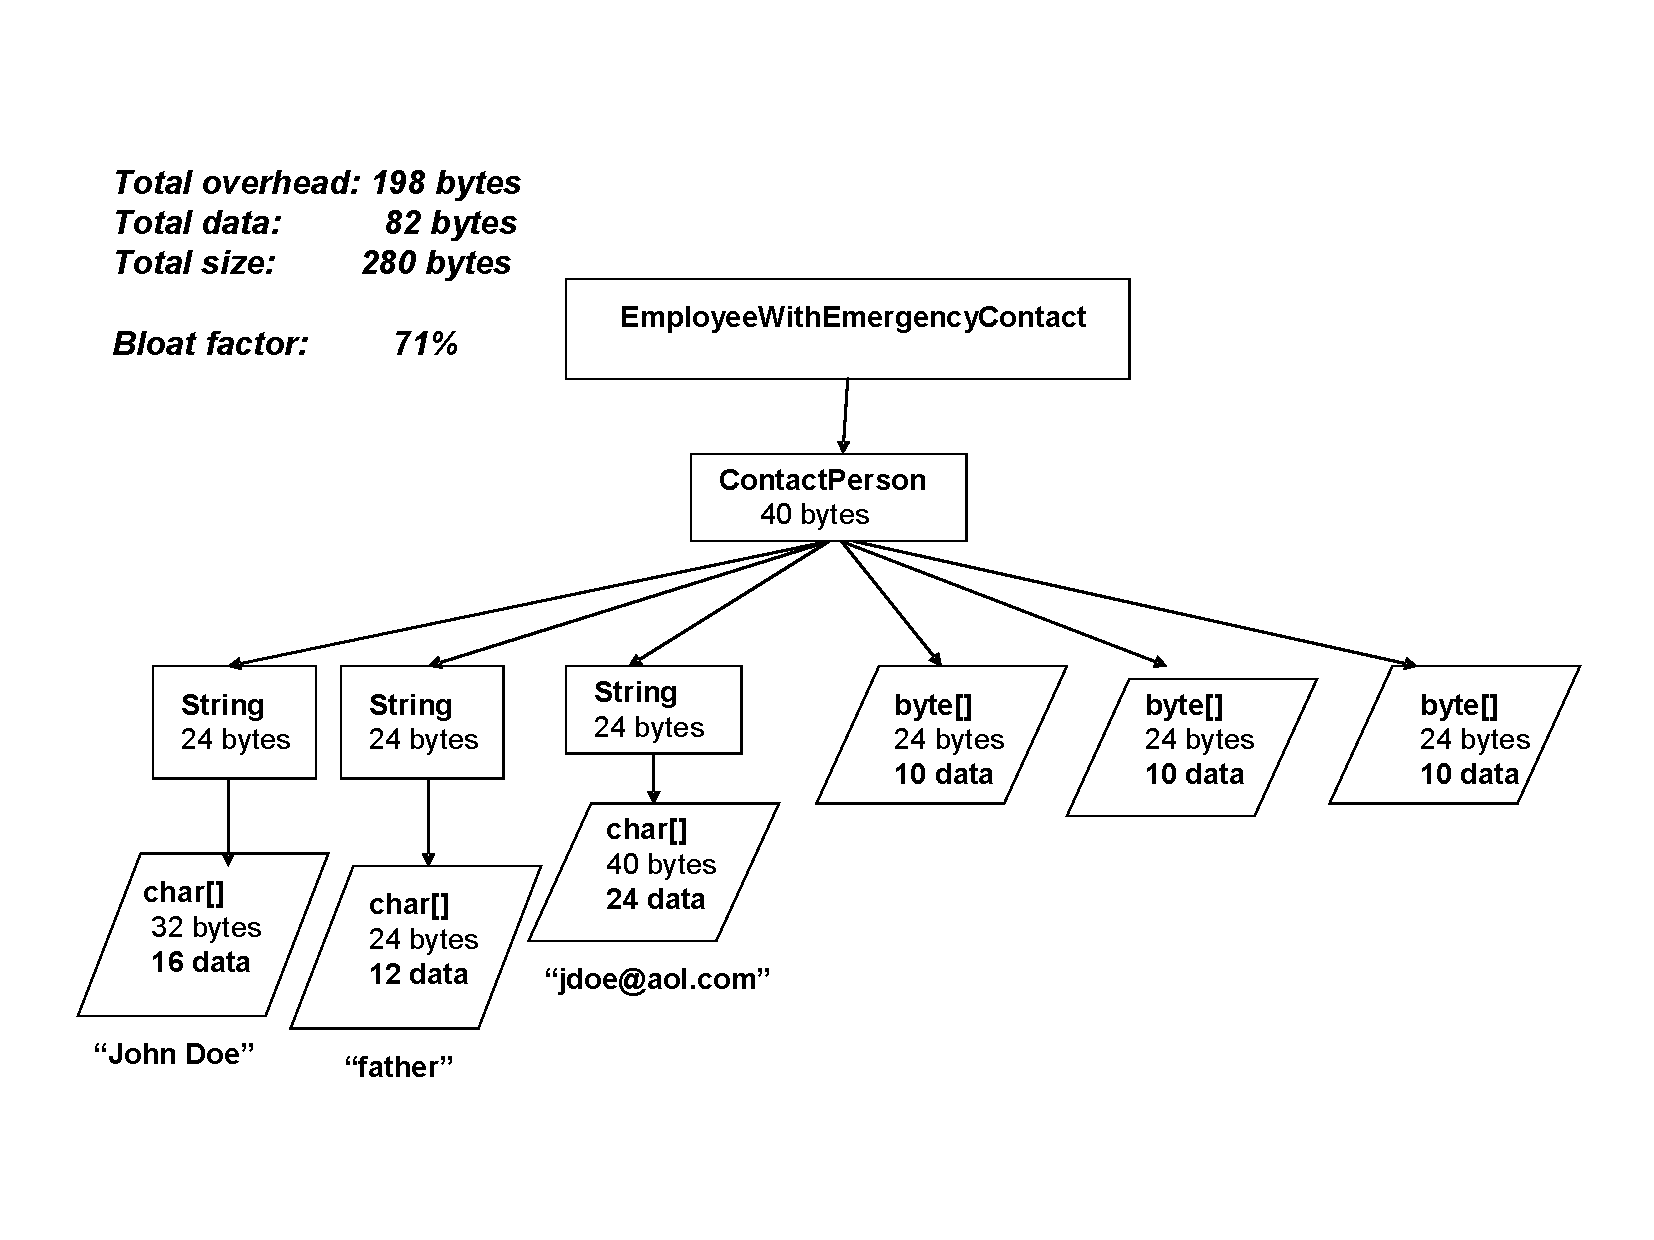
\includegraphics[width=.70\textwidth]{Figures/chapter4/refactored-fine-grain.pdf}
 % 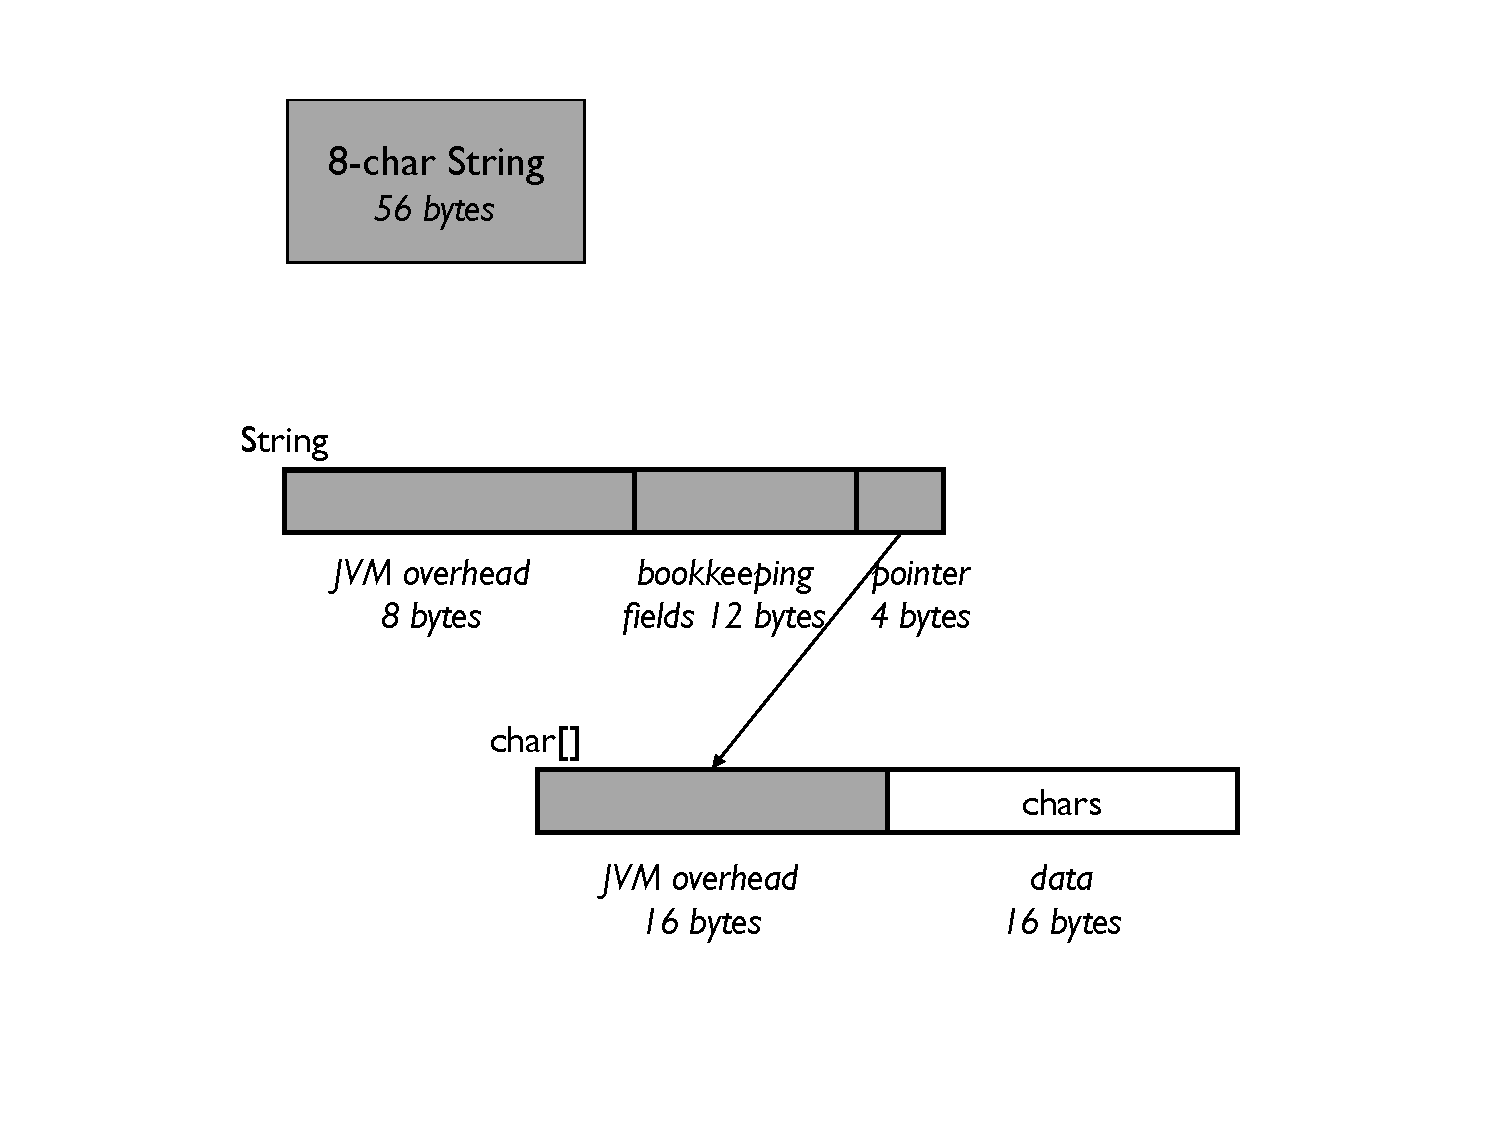
\includegraphics{eight-char-string}
  \caption{Memory layout for refactored emergency contact.}
  \label{fig:refactored-fine-grain}
\end{figure}

When many objects are used to represent one logical concept, this is an indication that the data model may be using too much delegation. Delegation is good, but it is possible to overuse a good thing.  A design with fewer, bigger objects has less overhead and is more scalable. Whenever you use delegation, there should be a good reason. This is especially true for the important data entities in an application, those that will determine the scalability of the program.  
 
\section{Large Base Classes}

As discussion in the last section, highly-delegated data models can result in too many small objects. Occasionally, you run across a highly-delegated data model where the delegated objects are large. This can happen when delegated classes inherit from a large base class. When fine grained data modeling is combined with inheriting from large base classes, memory costs multiply and can become prohibitive. 

\begin{example}[Keeping track of updates] 

A frequent data management requirement is to track creation and update information, that is, when data is created or updated and by whom.  Here is a base class, taken from a real application, that stores create and update information.  
\ttfamily
\begin{verbatim}
      class UpdateInfo {
         Date createDate;
         Party enteredBy;
         Date updateDate;
         Party updateBy;
      }
\end{verbatim}
\normalfont
You can track changes by subclassing from \texttt{UpdateInfo}. Update tracking is a \textit{cross-cutting feature}, since it can apply to any class in a data model.

\end{example}
Returning to Example 3 in Section~\ref{fine-grained-data-models}, suppose that updates to employee emergency contacts need to be tracked. You need to decide how precise the tracking should be. Should every update to every phone number and email address be tracked, or is it sufficient to track the fact that some contact information was changed for an emergency contact? If you decide to track changes to every contact phone number or email address, you can easily achieve this by extending the \texttt{ContactMethod} class defined in the fine-grained data model from Section~\ref{fine-grained-data-models}:
\ttfamily
\begin{verbatim}
      class ContactMethod extends UpdateInfo {
         ContactPerson owner;
      }
\end{verbatim}
\normalfont
Figure~\ref{fig:big-base-class} shows an instance of an contact person with update information associated with every \texttt{ContactMethod}. Not only is this a highly delegated structure with multiple \texttt{ContactMethod} objects, but each one has an additional 16 bytes. Furthermore, there are potentially four more objects of type \texttt{Date} and \texttt{Party} for each of the four \texttt{ContactMethod} objects. A far more scalable solution is to move up a level, and track changes to each \texttt{ContactPerson}. With this solution, you do not need such a fine-grained data model, and the update tracking functionality is 1/4 the cost.
\begin{figure}
  \centering
 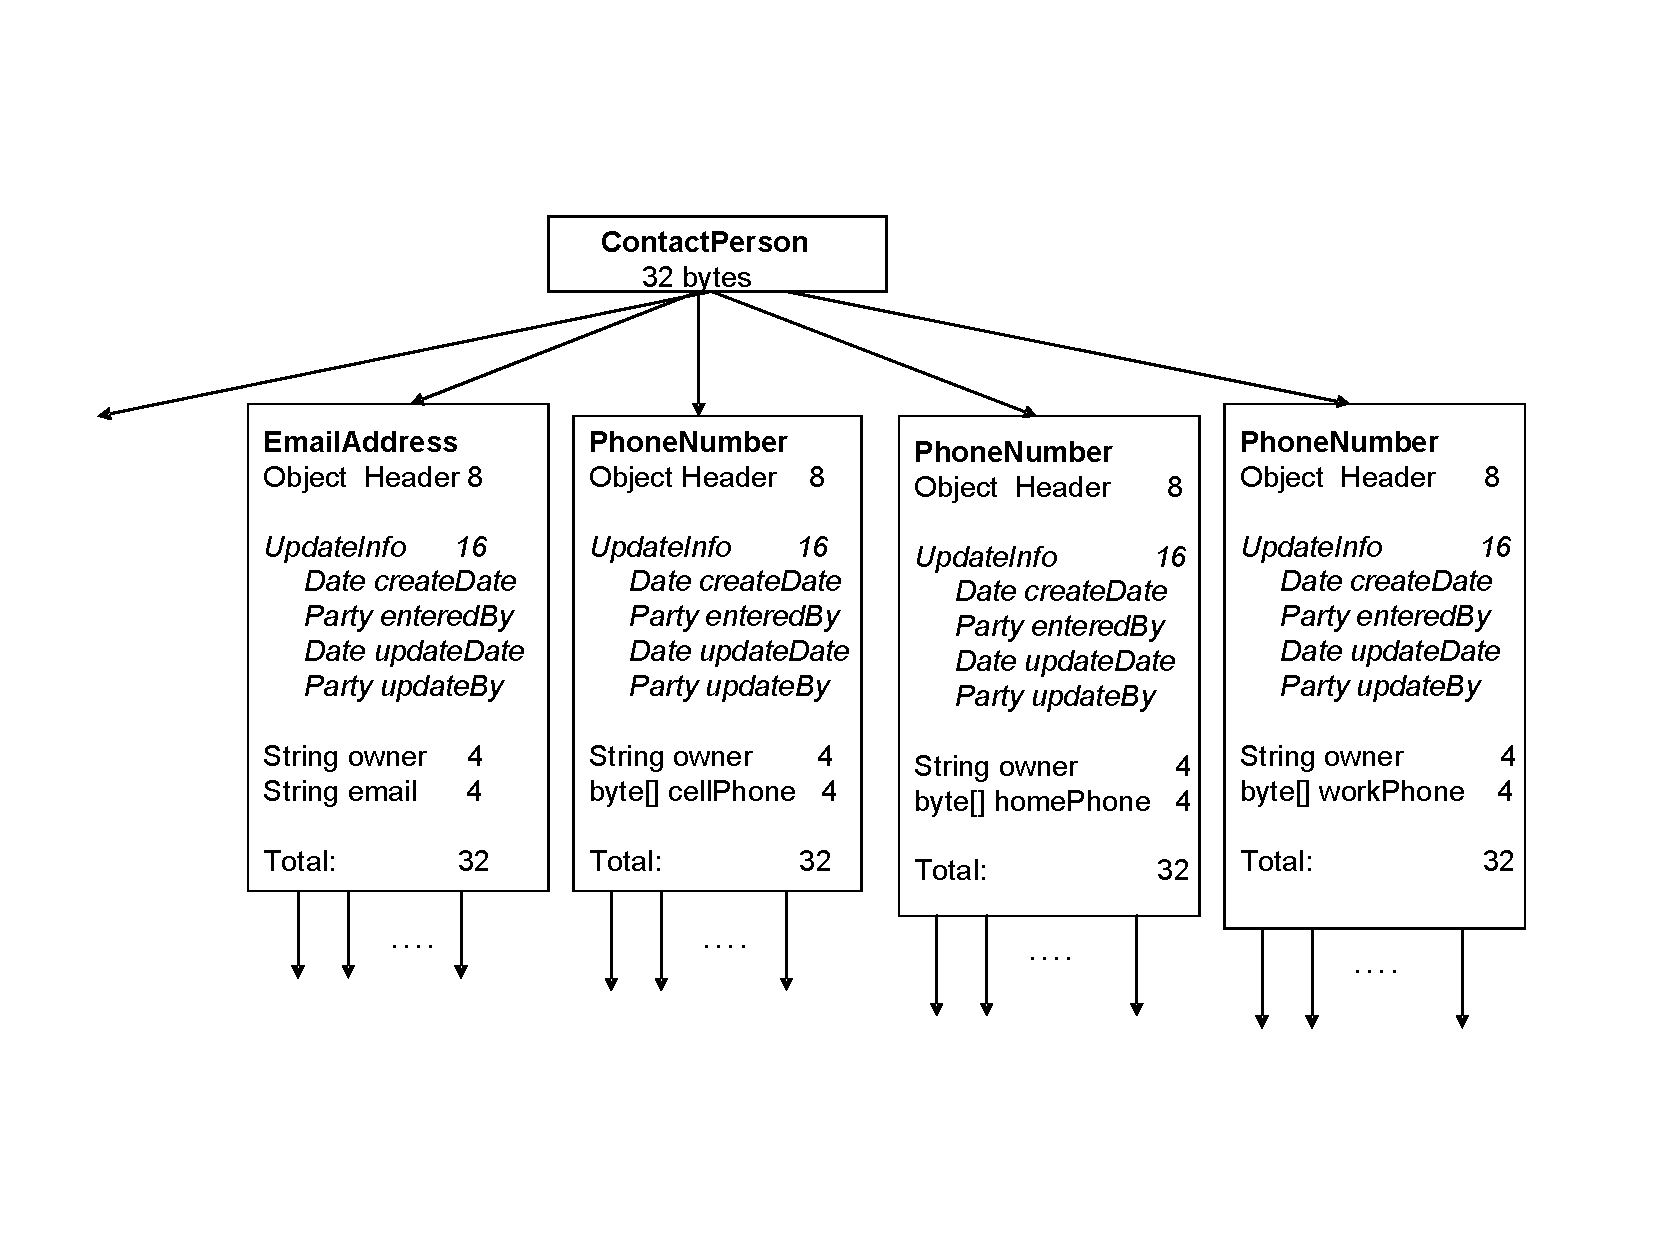
\includegraphics[width=.70\textwidth]{Figures/chapter4/big-base-class.pdf}
 % 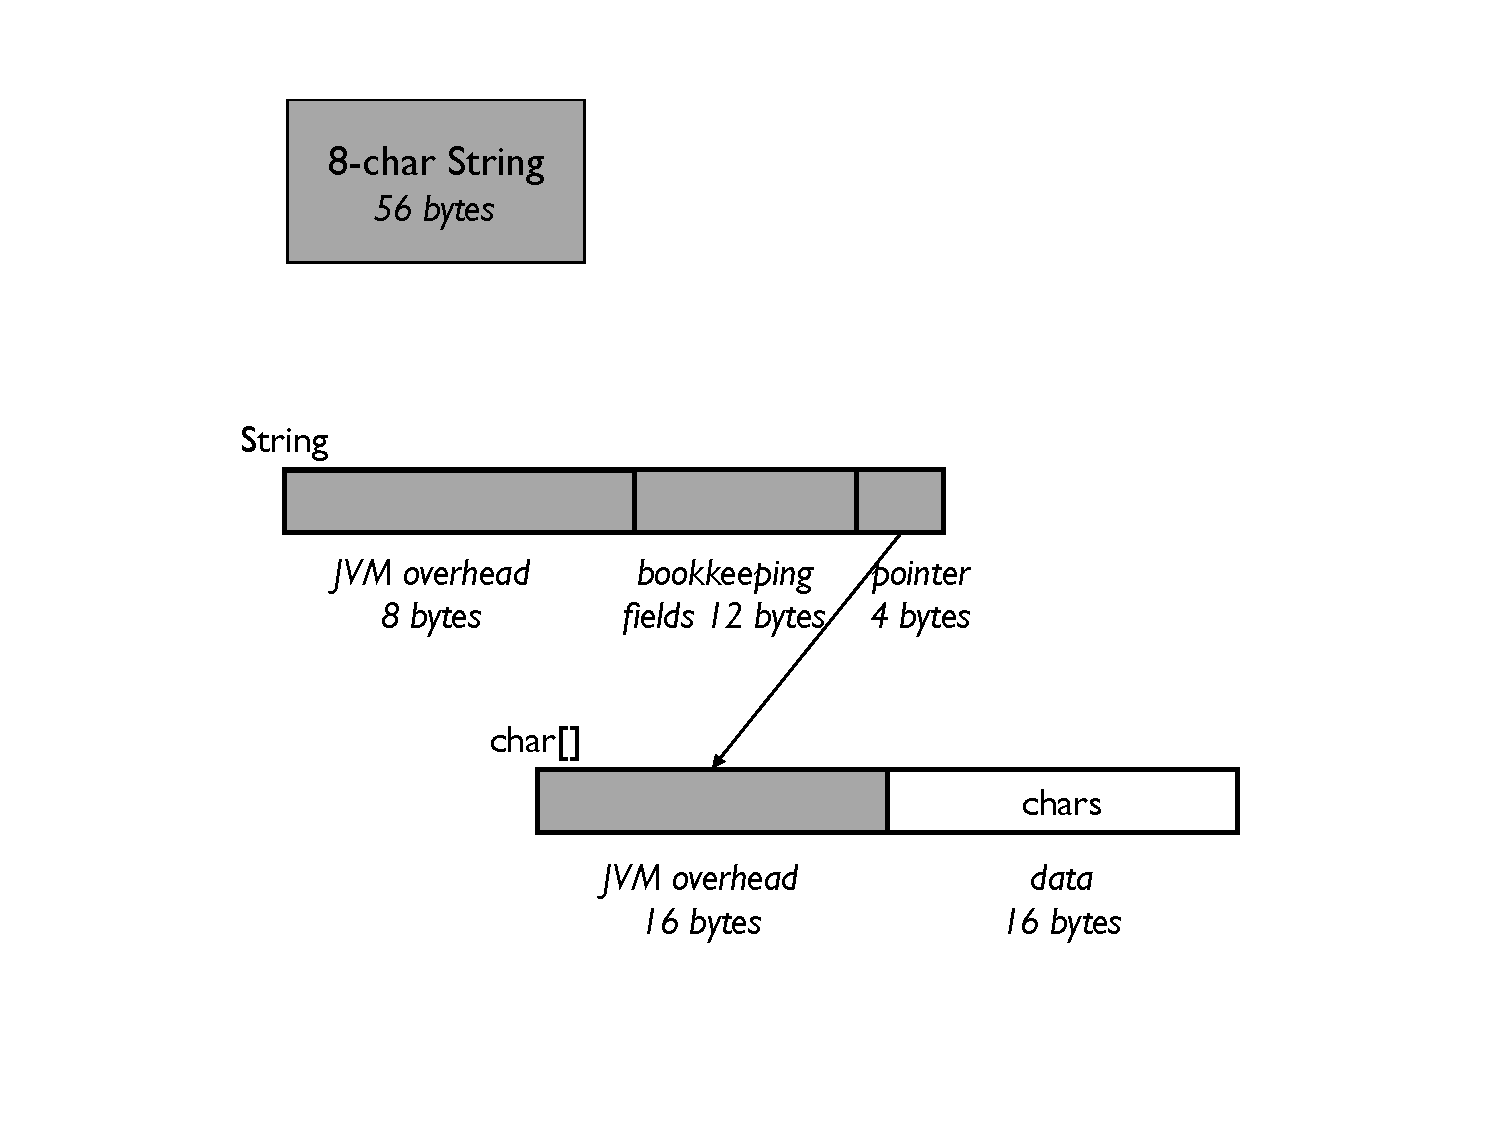
\includegraphics{eight-char-string}
  \caption{The cost of associating \texttt{UndateInfo} with every \texttt{ContactMethod}.}
  \label{fig:big-base-class}
\end{figure}
 
The solution in Figure~\ref{fig:big-base-class} provides a very fine granularity of functionality. An argument can be made in favor of this solution, since you lose functionality and flexibility if you only track updates to \texttt{ContactPerson}. However, if the program hits a scalabity problem, it may not be possible to be this casual with memory. Also, an alternate design may be available that gives the desired functionality in a more memory-efficient way. In this example, you could implement an update log instead of tracking updates in the objects themselves. Assuming updates are sparse, this is a much better solution. It is very easy define a subclass without looking closely at the memory size of a superclass, especially if the inheritance chain is long.   

\section{64-bit Architectures}

If your application does not fit into memory, perhaps moving to a 64-bit architecture will save you. However, to support a 64-bit address space, more memory is required. Object header sizes double, and pointers are 8 bytes instead of 4. Some studies~\cite{compressedAddress} show that memory consumption can increase by 40\%-50\% going from a 32-bit to a 64-bit address space for the same Java program.
\begin{example}[8-character string] 
Consider what happens to the 8-character string from Section~\ref{sec:bloat-def} in a 64-bit JRE. The memory layout is shown in Figure~\ref{fig:8-char-string-64-bit}. The 64-bit string is 50\% bigger than the 32-bit string. All of the additional cost is overhead.

\end{example} 
 \begin{figure}
  \centering
 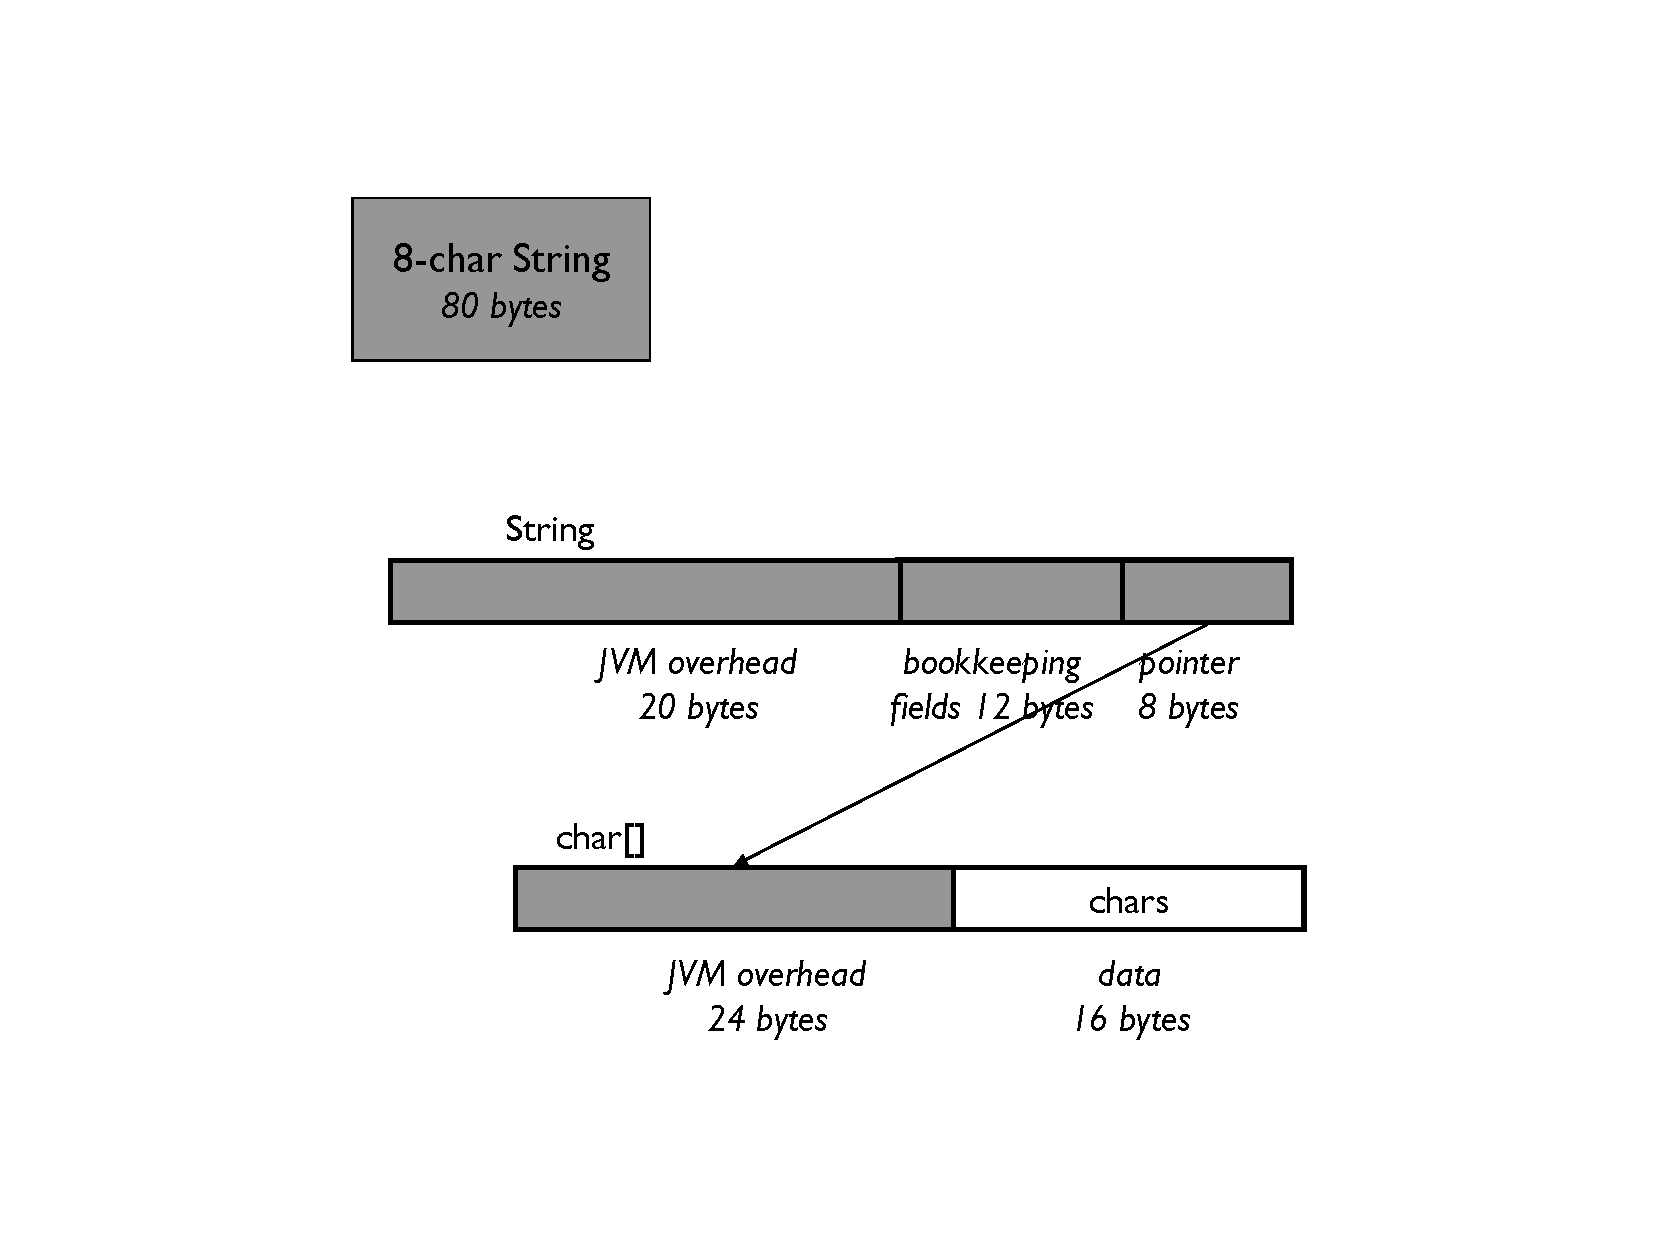
\includegraphics[width=.70\textwidth]{Figures/chapter4/8-char-string-64-bit.pdf}
 % 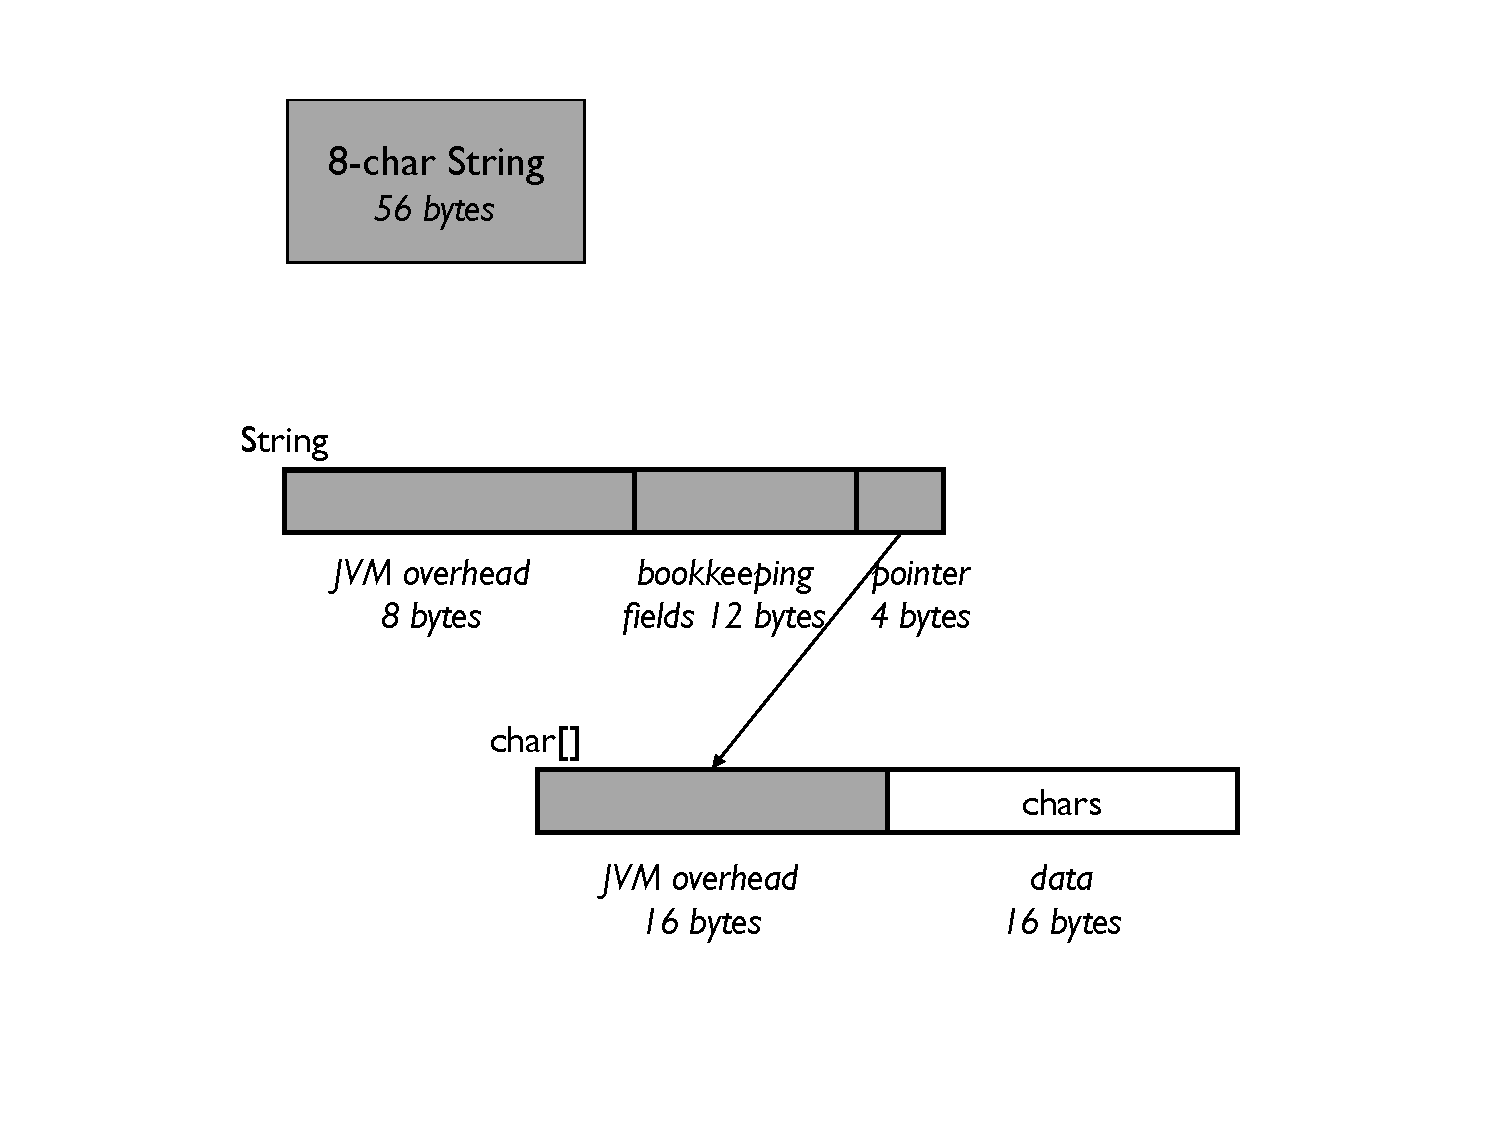
\includegraphics{eight-char-string}
  \caption{The memory layout for an 8 character string by a 64-bit JRE}
  \label{fig:8-char-string-64-bit}
\end{figure}

In reality, things are not so bad. Both the Sun and the IBM JREs have implemented a scheme for compressing addresses that avoids this code size blowup, provided that the heap is less than 32 gigabytes. Address compression is implemented by stealing a few unused bits from 32-bit pointers. During execution, 32-bit compressed addresses are converted into 64-bit native addresses, and vice-versa. 

Address compression is available in the Sun Java 6 (update 14) release, enabled with the option -XX:+UseCompressedOops. It is available in IBM Java 6 J9 SR 4 with the option -Xcompressedrefs.

\section{Summary}

%An entity is modeled by a set of interrelated classes. This chapter describes how to estimate the size of an instantiated entity, using rules for estimating the size of basic objects. During the modeling process, programmers choose how many classes to define.
The decision to delegate functionality to another object sometimes involves making a tradeoff between flexibility and memory cost. You need to decide how much flexibility is really needed, and you also need to be aware of the actual memory costs. This chapter provides the basic knowledge for estimating memory costs. 
\begin{itemize}
\item An object size depends on the object header size, field alignment, object alignment, and pointer size. These can vary, depending on the JRE and the hardware. The minimum size of an object is the sum of the header and the field type sizes, rounded up to the alignment boundary. This is a good way to estimate objects for the Sun JRE.
\end{itemize}
If you need the exact size of objects, there are various tools available. A list of resources is provided in the Appendix.

This chapter also describes several costly anti-patterns to avoid.
\begin{itemize}
\item A \textit{highly-delegated data model} results in too many small objects and a large bloat factor. Typically, each object has only a few fields, which is excessive data granularity.  
\item A \textit{highly-delegated data model with large base classes} results in too many big objects. Often, the data model is providing a fine granularity of function, which may no be needed.
\end{itemize}   

Both the design of Java and software engineering best practices encourage highly delegated data models with many objects. This cost is often considered to be insignificant --- delegating to another object is just a single level of indirection. But the costs of the pointers and object headers needed to implement delegation indirection add up quickly, and contribute significantly to large bloat factors in real applications. 

  

